\documentclass[10pt,a4paper]{article}
\usepackage{ucs}
\usepackage[utf8x]{inputenc}
\usepackage[ngerman]{babel}
\selectlanguage{ngerman}
\usepackage[T1]{fontenc}

% Math stuff
\usepackage{amsmath}
\usepackage{amsfonts}
\usepackage{amssymb}

% Farben
\usepackage[usenames,x11names,dvipsnames,rgb]{xcolor}
\definecolor{grey}{rgb}{0.4,0.4,0.4}
\definecolor{lightgrey}{rgb}{0.8,0.8,0.8}
\definecolor{ultralightgrey}{rgb}{0.96,0.96,0.96}

% Grafix
\usepackage{graphicx}

% TikZ (dot2tex etc.) - brauchen wir zurzeit nicht
% \usepackage{tikz}
% \usetikzlibrary{decorations, arrows, shapes}

% Captions in minipages
\usepackage{capt-of}

% Farben in Tabellen
\usepackage{colortbl}

% Lange Tabellen
\usepackage{longtable}

% Gewrappte boxen (können innerhalb f{rame}box's verwendet werden)
\usepackage{minibox}

% FloatBarrier stellt sicher, dass das Literaturverzeichnis am Ende des
% Dokuments erscheint.
\usepackage{placeins}

% Hyperref
\usepackage{hyperref}
% Hypersetup
\hypersetup{
    pdftitle = {Semesterarbeit Kryptographie - Gruppenarbeit PKCS},
    pdfauthor = {Aregger Thomas, Gutknecht Jürg, Dünki Marc, Daniel David},
    pdfsubject = {Semesterarbeit Kryptographie - Gruppenarbeit PKCS},
    pdfkeywords = {Kryptographie PKCS Semesterarbeit Gruppenarbeit},
    % hidelinks
    colorlinks = true,
    linkcolor = blue,
    % urlcolor = black
    urlcolor = Blue,
    citecolor = grey
}

\urlstyle{same}

\title{Semesterarbeit Kryptographie - Gruppenarbeit  PKCS}
\author{
    Aregger Thomas \small{thomas.aregger@students.ffhs.ch}\\
    Dünki Marc \small{marc.duenki@students.ffhs.ch}\\
    Gutknecht Jürg \small{juerg.gutknecht@students.ffhs.ch}\\
    Daniel David \small{david.daniel@students.ffhs.ch}
}

\date{\today}

\begin{document}

\maketitle
\tableofcontents

\section{Einleitung}
Dieses Dokument liefert einen Überblick über das Themengebiet der Public-Key Cryptography
Standards und entstand als Teil der Semesterarbeit des Moduls Kryptologie bei Herrn Josef
Schuler.

\subsection{Gruppe}
Die Gruppe der an dieser Arbeit mitwirkenden Studenten umfasst:
\begin{itemize}
   \item Thomas Aregger
   \item David Daniel
   \item Marc Dünki (Projektleiter)
   \item Jürg Gutknecht
\end{itemize}

\subsection{Vorgehensweise}

\begin{minipage}[t]{\textwidth}
    \centering
    \begin{tabular}{|l|p{7.8cm}|} \hline
        \textbf{Datum} & \textbf{Fortschritt} \\\hline
        7.9.2013 & Gruppenbildung \\\hline
        8.9.2013 - 4.10.2013 & Individuelles Erarbeiten der Aufgabenstellung \\\hline
        4.10.2013 & Aufteilen der Themen innerhalb der Gruppe \\\hline
        4.10.2013 - 28.12.2013 & Individuelles Bearbeiten der Inhalte gemäss
        Themenverteilung \\\hline
        28.12.2013 & Besprechen des Fortschritts \\\hline
        28.12.2013 - 4.1.2014 & Individuelles Finalisieren der Inhalte gemäss
        Themenverteilung \\\hline
        4.1.2014 & Verteilen der Aufgaben zum Abschliessen der Arbeit \\\hline
        4.1.2014 - 9.1.2014 & Abschliessen der Arbeit \\\hline
        & Abgabe der Arbeit \\\hline
    \end{tabular}
    \captionof{table}{Vorgehensweise}
    \label{tab:vorgehensweise}
\end{minipage}

\subsection{Arbeitsteilung}

\subsubsection{Verteilung der Themen}
\begin{minipage}[t]{\textwidth}
   \centering
   \begin{tabular}{|c|l|} \hline
      \textbf{PKCS\#} & \textbf{Person} \\\hline
      1 & Thomas Aregger \\\hline
      3 & Marc Dünki \\\hline
      5 & Thomas Aregger \\\hline
      6 & Jürg Gutknecht \\\hline
      7 & David Daniel \\\hline
      8 & Thomas Aregger \\\hline
      9 & David Daniel \\\hline
      10 & Jürg Gutknecht \\\hline
      11 & Jürg Gutknecht \\\hline
      12 & Marc Dünki \\\hline
      13 & David Daniel \\\hline
      15 & Marc Dünki \\\hline
   \end{tabular}
   \captionof{table}{Verteilung der Themen}
   \label{tab:arbeitsteilung}
\end{minipage}

\subsubsection{Weitere Aufgaben}
\begin{minipage}[t]{\textwidth}
   \centering
   \begin{tabular}{|p{7.4cm}|l|} \hline
      \textbf{Aufgabe} & \textbf{Person} \\\hline
      Zusammenführung der Beiträge in einem Dokument & David Daniel \\\hline
      Zusammenfassung der Beiträge in einer Präsentation & Alle (jeder seinen Teil) \\\hline
      Abgabe der Aufgabe & Thomas Aregger \\\hline
   \end{tabular}
   \captionof{table}{Verteilung weiterer Aufgaben}
   \label{tab:weitere-aufgaben}
\end{minipage}

\section{Public-Key Cryptography Standards}
Die Public Key Cryptography Standards (PKCS) sind eine von RSA Laboratories~\cite{rsa-lab}
seit den 1990er-Jahren veröffentlichte Reihe an Standards zum Themengebiet der
asymmetrischen Kryptographie (Public-Key Kryptographie).

Die Gruppe der PKCS besteht aus den nachfolgend aufgelisteten Standards, welche in diesem
Kapitel detailliert betrachtet werden.

\begin{table}[ht]
    \centering
    \begin{tabular}{|c|l|} \hline
        \textbf{PKCS \#} & \textbf{Titel} \\\hline
        1 & RSA Cryptography Standard \\\hline
        3 & Diffie-Hellman Key-Agreement Standard \\\hline
        5 & Password-Based Cryptography Standard \\\hline
        6 & Extended-Certificate Syntax Standard \\\hline
        7 & Cryptographic Message Syntax Standard \\\hline
        8 & Private-Key Information Syntax Standard \\\hline
        9 & Selected Object Classes and Attribute Types \\\hline
        10 & Certification Request Syntax Standard \\\hline
        11 & Cryptographic Token Interface Standard \\\hline
        12 & Personal Information Exchange Syntax \\\hline
        13 & Elliptic Curve Cryptography Standard \\\hline
        14 & Pseudo Random Number Generation \\\hline
        15 & Cryptographic Token Information Syntax Standard \\\hline
    \end{tabular}
    \caption{Übersicht der PKCS}
    \label{tab:pkcs-overview}
\end{table}

Die PKCS \#2 und \#4 wurden in den PKCS \#1 überführt und sind nicht mehr eigener Bestandteil
der PKCS-Familie~\cite[S.1]{kal91}.

PKCS \#14 befindet sich zur Zeit in Entwicklung, wird auf den PKCS-Seiten der RSA
Laboratories~\cite{pkcs-standards} nicht erwähnt und wird hier ebenfalls nicht genauer
betrachtet.

\subsection{PKCS \#1: RSA Cryptography Standard}

Das PKCS Dokument \#1 gibt Empfehlungen zur Implementierung von Public Key Kryptografie
auf Basis des RSA Algorithmus. Dabei werden hauptsächlich die folgenden Aspekte abgedeckt,
welche nachfolgend genauer erläutert werden:

\begin{itemize}
    \item Kryptografische Primitive
    \item Verschlüsselungs Schemas (Encryption schemes)
    \item Signierungs Schemas (Signature schemes)
\end{itemize}

\subsubsection{Key Typen}

Bei RSA existieren 2 unterschiedliche Key Typen, welche zusammen als RSA Key Pair
bezeichnet werden:

\begin{itemize}
    \item \textit{RSA Public Key} wird zum verschlüsseln bzw. verifizieren benutzt.
    \item \textit{RSA Private Key} wird zum entschlüsseln bzw. signieren benutzt.
\end{itemize}

\subsubsection{RSA Public Key}
\label{sec:rsa-public-key}
Der Public Key besteht aus zwei Komponenten, nämlich einem Modulo und einem öffentlichen
Exponenten (Public exponent). Beides sind positive Integer.

\begin{description}
    \item[n =] RSA Modulo. Der Modulo ist ein Produkt von mindestens 2 Primzahlen. In
        Lehrbüchern und Beispielen werden häufig nur 2 Primzahlen multipliziert, es können
        aber auch mehr verwendet werden. $(r_1, r_2, \dots, r_3)$ $r_1$ und $r_2$ werden
        häufig auch als $p$ und $q$ bezeichnet.
    \item[e =] Public exponent. Zahl zwischen 3 und $n-1$, welche relativ Prim
        (teilerfremd) zu $(r_1 - 1) * (r_2 -1) * (r_3 - 1)$ ist.
\end{description}

Der Einfachheit halber wird in dieser Zusammenfassung immer davon ausgegangen, dass bei
der Generierung von n nur 2 Primzahlen verwendet wurden.

\subsubsection{RSA Private Key}
Der Private Key besteht aus dem selben Modulo $n$ wie der Public Key. Zusätzlich existiert
ein privater Exponent $d$:

\begin{description}
    \item[n =] RSA Modulo (siehe Kapitel~\ref{sec:rsa-public-key} (RSA Public Key)).
    \item[d =] Private Exponent. $e * d \equiv 1 \mod (p - 1)(q - 1)$. $d$ ist also das
        Inverse von $e \mod (p - 1)(q - 1)$.
\end{description}

\begin{description}
    \item[Bemerkung:] Würden mehr als 2 Primzahlen verwendet werden, würde der Private Key
        noch einige Komponenten mehr enthalten.
\end{description}

\subsubsection{Kryptographische Primitive}
Kryptographische Primitive bezeichnen grundlegende mathematische Operationen auf denen die
kryptographischen Schemas aufbauen. Es werden 4 Typen von Primitiven spezifiziert:
\begin{itemize}
    \item Verschlüsselung \& Entschlüsselung
    \item Signierung und Verifikation
\end{itemize}

\paragraph{Verschlüsselungs und Entschlüsselungs Primitive}
Ein Verschlüsselungsprimitiv erstellt unter Verwendung des Public Keys aus einer Nachricht
ein Chiffrat. Das Entschlüsselungsprimitiv gewinnt unter Verwendung des Private Keys
wieder die Nachricht aus dem Chiffrat.  RSA definiert die beiden Schemes RSAEP und RSADP
(RSA Encryption/Decryption Primitiv).  Beide verwenden die selben mathematischen
Operationen, wobei einfach unterschiedlicher Input verwendet wird.

\vspace{0.5cm}
\begin{minipage}[t]{0.8\textwidth}
    \begin{tabular}{lll}
        \textbf{RSAEP} & & \\
        Input & $(n, e)$ & Public Key \\
        & $m$ & Nachricht \\
        Output & $c$ & Chiffrat
    \end{tabular}
\end{minipage}

\vspace{0.5cm}
\begin{minipage}[t]{0.8\textwidth}
    \begin{tabular}{lll}
        \textbf{RSADP} & & \\
        Input & $(n, d)$ & Private Key \\
        & $c$ & Chiffrat \\
        Output & $m$ & Nachricht
    \end{tabular}
\end{minipage}
\vspace{0.5cm}

Für die genaue Berechnung sei auf PKCS \#1~\cite[Kapitel 5.1]{pkcs1} verwiesen.

\paragraph{Signatur und Verifikation Primitive}
Das Signatur Primitiv erstellt unter Verwendung des Private Keys aus einer
Nachricht~\footnote{Wie später noch gezeigt wird, muss es sich bei der
Nachricht nicht um den gleichen Text handeln wie bei der Verschlüsselung.  Es
kann z.Bsp. auch der Hashwert der verschlüsselten Nachricht sein.} eine
Signatur. Das Verifikations Primitiv gewinnt unter Verwendung des Public Keys
aus der Signatur wieder die Nachricht. Die Primitiven RSASP1 und RSAVP1 (RSA
Signature/Verification Primitives) funktionieren gleich wie RSADP und RSAEP,
mit dem einzigen Unterschied, dass die Input und Output Argumente
unterschiedlich sind.

\vspace{0.5cm}
\begin{minipage}[t]{0.8\textwidth}
    \begin{tabular}{lll}
        \textbf{RSASP1} & & \\
        Input & $(n, d)$ & Private Key \\
        & $m$ & Nachricht \\
        Output & $s$ & Signatur
    \end{tabular}
\end{minipage}

\vspace{0.5cm}
\begin{minipage}[t]{0.8\textwidth}
    \begin{tabular}{lll}
        \textbf{RSAVP1} & & \\
        Input & $(n, e)$ & Public Key \\
        & $s$ & Signatur \\
        Output & $m$ & Nachricht
    \end{tabular}
\end{minipage}

\subsubsection{Schemas}
Ein Schema kombiniert kryptographische Primitive mit anderen Techniken um ein bestimmtes
Schutzziel zu erreichen. In PKCS \#1 werden Verschlüsselungs und Signatur Schemas
spezifiziert. Die Schemas definieren nur die Schritte welche unternommen werden um die
Daten zu verarbeiten. Es wird z.Bsp. keine Schlüssel generiert oder validiert.

\subsubsection{Verschlüsselungs Schemas}
Ein Verschlüsselungs Schema besteht aus einer Verschlüsselungs- und einer Entschlüsselungs
Operation. Ein solches Schema kann für verschiedene Zwecke verwendet werden. Häufig wird
es verwendet um z.Bsp. einen symmetrischen Schlüssel auszutauschen. In PKCS \#1 werden
zwei unterschiedliche Schemas spezifiziert. RSAES-OAEP und RSAES-PKCS1-v1\_5. Für neuere
Applikationen sollte nur noch ersteres verwendet werden, deshalb wird das letztere hier
nicht weiter berücksichtigt.

Grundsätzlich wird bei den Schemas zuerst ein Encoding der Nachricht durchgeführt. Die
codierte Nachricht wird dann in eine Integerversion der Nachricht konvertiert. Auf diese
Integerversion der Nachricht wird anschliessend die Verschlüsselungs Primitve angewendet
um das Chiffrat zu erstellen. Genau umgekehrt funktioniert das Verfahren um wieder den
Klartext zu erhalten.

\paragraph{RSAES-OAEP}
RSAES-OAEP kombiniert die RSAEP/RSADP Primitive mit der EME-OAEP Encoding Methode. OAEP
steht für Optimal Asymmetric Encryption Padding und dient dazu das Kryptosystem gegen
Chosen-Plaintext Attacken zu schützen in dem bei jeder Nachricht ein Zufalls-Padding
vorgenommen wird. Dieses sehr wichtige Padding wird im Schulbuch RSA selten erwähnt.
Um den Rahmen dieses Dokumentes nicht zu sprengen, wird im folgenden nur die
Verschlüsselung beschrieben. Die Entschlüsselung funktioniert nach einem ähnlichen
Prinzip.

\subparagraph{Grobes Verfahren:}
\begin{enumerate}
    \item Länge der Nachricht prüfen
    \item Encoding vornehmen (Details siehe EME-OAEP~\ref{par:eme-oaep})
    \item Konvertieren in Integer Version, mithilfe von OS2IP (Octet String to Integer
        Primitive)
    \item Anwenden der RSAEP Primitive
\end{enumerate}

\subparagraph{EME-OAEP}
\label{par:eme-oaep}
\begin{enumerate}
    \item Generieren des Hashwertes lHash des Labels L~\footnote{In PKCS \#1 werden für
        RSAES-OAEP lediglich die Hashfunktionen SHA-1 und SHA-256/384/512 empfohlen.}
        (welches in dieser Version der Spezifikation leer ist. Somit wird hier immer der
        gleiche Hashwert verwendet, welcher jedoch natürlich abhängig von der verwendeten
        Hashfunktion ist)
    \item Generieren eines Null Oktet Strings PS der Länge k - mLen - 2hLen
    \item Zusammenfügen von lHash, PS, einem Oktet $\mathtt{0x01}$ und der Nachricht M.
        Wird zusammen als data block DB bezeichnet.
    \item Generieren eines Random Strings seed
    \item Anwenden einer MGF~\footnote{MGF = Mask Generation Functions werden hier nicht
        näher erläutert. Für Details sei auf das Kapitel B.2 in PKCS \#1 verwiesen} auf
        dem seed. Output = dbMask
    \item maskedDB = DB xor dbMask
    \item Anwenden einer MGF auf maskedDB. Output = seedMask
    \item maskedSeed = seed xor seedMask
    \item Das Oktet $\mathtt{0x00}$, maskedSeed und maskedDB bilden zusammen die codierte
        Nachricht.
\end{enumerate}

\begin{minipage}[t]{0.8\textwidth}
    \begin{tabular}{ll}
        k & Länge des Modulo n \\
        mLen & Länge der Nachricht \\
        hLen & Länge des Hashwertes
    \end{tabular}
\end{minipage}

\begin{figure}[ht]
    \centering
    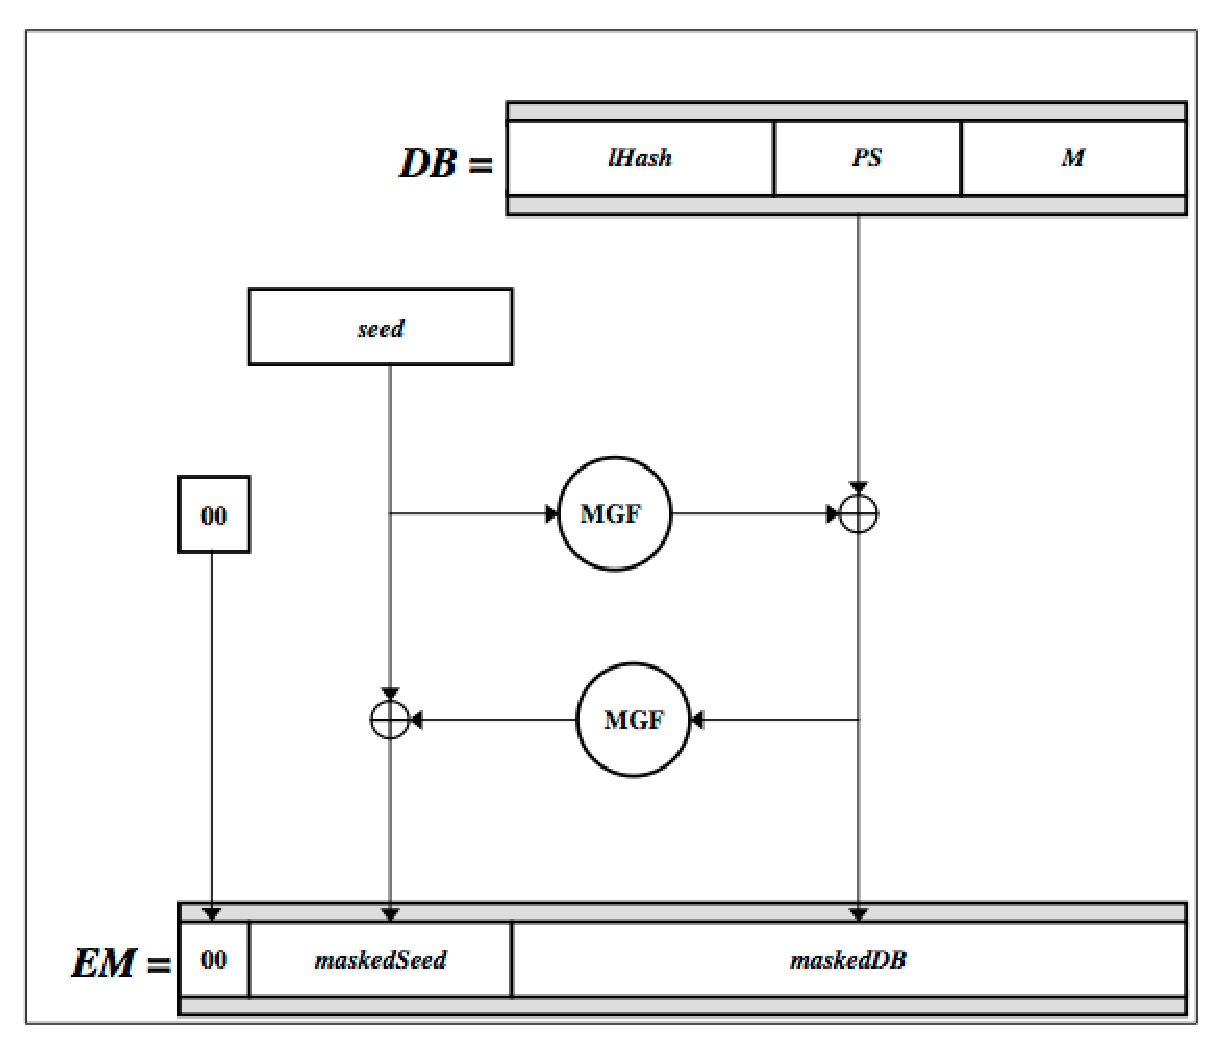
\includegraphics[scale=0.48]{images/eme-oap-graph}
    \caption{Grafische Ansicht des EME-OAEP. \small{Quelle: PKCS \#1}}
    \label{fig:eme-oap-graph}
\end{figure}

\subsubsection{Signatur Schemas}
Ein Signatur Schema besteht aus einer \textit{signature generation operation} und einer
\textit{signature verifcation operation}. Die Erstere wird von der unterzeichnenden Partie
mit Hilfe seines privaten Schlüssels verwendet um eine Signatur zu erstellen. Letztere
wird von der prüfenden Partie mit Hilfe des öffentlichen Schlüssels der unterzeichnenden
Partie verwendet um die Signatur zu überprüfen. Die in PKCS \#1 spezifizierten Schemas
werden auch als Signatur Schemas mit Anhang bezeichnet, da sie die Nachricht selbst
ebenfalls benötigen um die Signatur zu verifizieren. Im Gegensatz dazu existieren auch
Signatur Schemas mit Möglichkeit zur Nachricht-Wiederherstellung.

In PKCS\#1 werden zwei Schemas spezifiziert. RSASSA-PSS und RSASSA-PKCS1-v1\_5. Für neuere
Applikationen wird RSASSA-PSS empfohlen, weshalb in diesem Dokument nur auf dieses
eingegangen wird.

\paragraph{RSASSA-PSS}
RSASSA-PSS kombiniert die Primitive RSASP1/RSAVP1 mit dem EMSA-PSS Encoding (Auf EMSA-PSS
wird in diesem Dokument nicht näher eingegangen). RSASSA-PSS ist probabilistisch da ein
zufallsgeneriertes Salt eingefügt wird (PSS = Probabilistic Signature Scheme). Die
Sicherheit beruht jedoch nicht auf diesem Salt und kann immer noch als gewährleistet
betrachtet werden, wenn ein solcher Salt nicht generiert werden kann.

\par\vspace{0.5cm}
\textbf{Signature generation operation}
\par\vspace{0.5cm}
\begin{minipage}[t]{0.8\textwidth}
    \begin{tabular}{lll}
        Input & $K$ & Private Key der signierenden Partie \\
        & $M$ & Nachricht \\
        Output & $S$ & Signatur
    \end{tabular}
\end{minipage}
\par\vspace{0.5cm}

\textbf{Schritte:}
\begin{enumerate}
    \item Anwenden des Encodings EMSA-PSS-ENCODE
    \item Konvertieren der codierten Nachricht in Integer (OS2IP)
    \item Anwenden von RSASP1 Primitive mit Hilfe von K und M
    \item Konvertieren Integer Version in Oktet-String (I2OSP)
    \item Output von Signatur S
\end{enumerate}

\par\vspace{0.5cm}
\textbf{Signature verification operation}
\par\vspace{0.5cm}
\begin{minipage}[t]{0.8\textwidth}
    \begin{tabular}{lll}
        Input & $(n, e)$ & Public Key der signierenden Partie \\
        & $M$ & Nachricht \\
        Output & & valide/invalide Signatur
    \end{tabular}
\end{minipage}
\par\vspace{0.5cm}

\textbf{Schritte:}
\begin{enumerate}
    \item Prüfung der Signatur Länge (Muss gleich Lang wie der Modulo n sein)
    \item Konvertieren der Signatur S in Integer (OS2IP)
    \item Anwenden der RSAVP1 Primitive mit Hilfe vom Public Key (n,e) und der
        Nachricht M.
    \item Konvertieren in Oktet-String (I2OSP)
    \item Verifikation mittels EMSA-PSS-VERIFY
    \item Ouput valide/invalide Signatur
\end{enumerate}

Bei der Verifikation wird zuerst der Salt wiederhergestellt, danach der Hashwert erneut
berechnet und mit dem Hashwert welcher in der Signatur enthalten ist verglichen. Bei
Übereinstimmung ist die Signatur valide.

Die Abbildung~\ref{fig:emsa-pss-encoding} illustriert das EMSA-PSS-ENCODING.

\begin{minipage}[t]{0.8\textwidth}
    \centering
    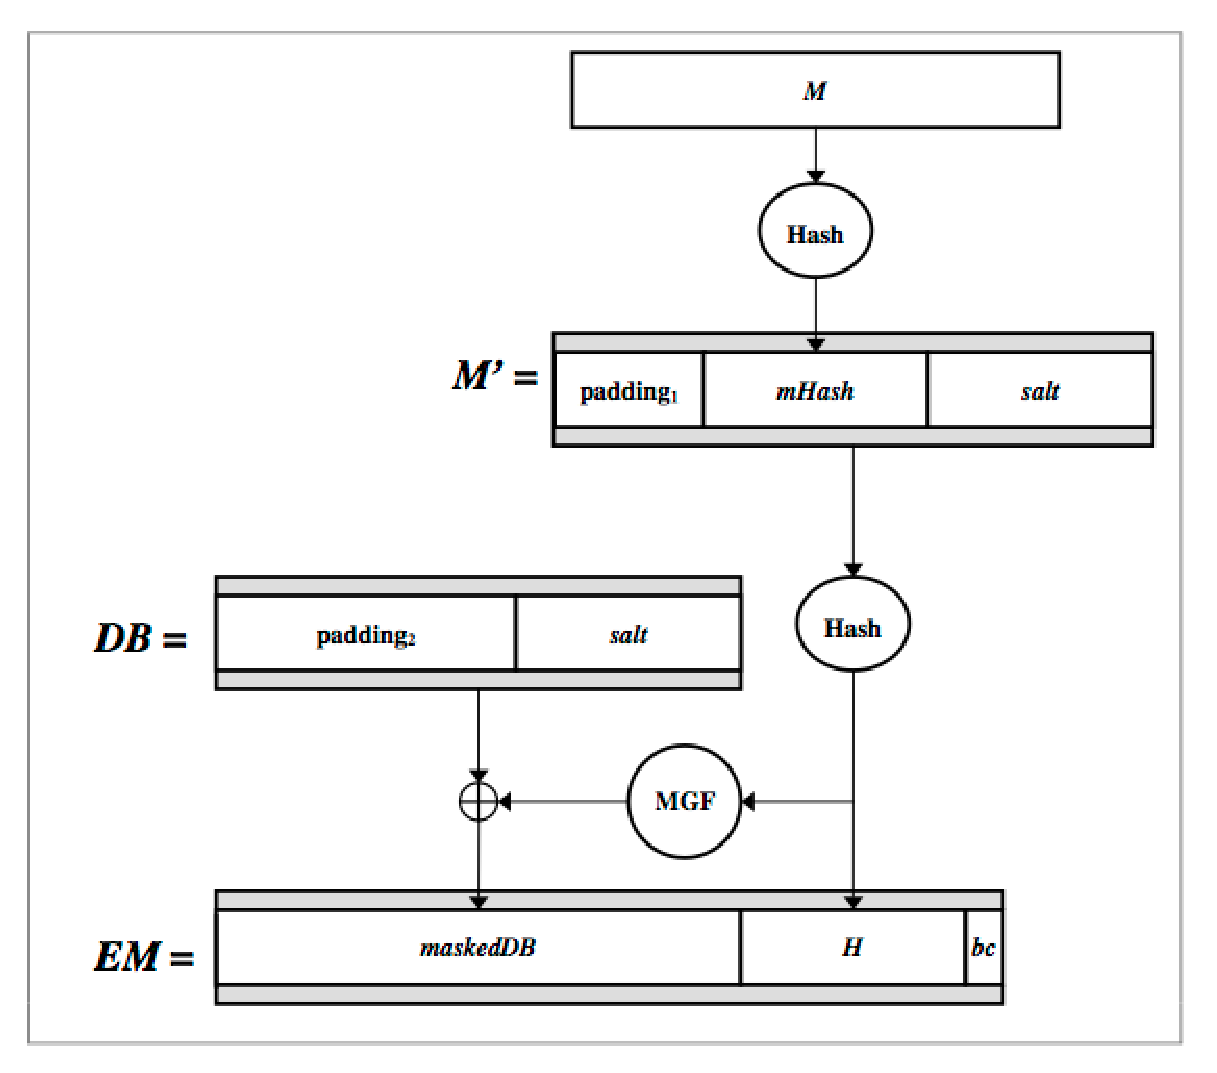
\includegraphics[scale=0.48]{images/emsa-pss-encoding}
    \captionof{figure}{EMSA-PSS-ENCODING. \small{Quelle: PKCS \#1}}
    \label{fig:emsa-pss-encoding}
\end{minipage}

\subsection{PKCS \#3: Diffie-Hellman Key-Agreement Standard}

\subsubsection{Einleitung}
\begin{table}[ht]
    \centering
    \begin{tabular}{|l|p{6.4cm}|} \hline
        Aktuelle Version des Standards & 1.4 \\\hline
        Datum & Revised November 1, 1993 \\\hline
        Seitenzahl & 8 \\\hline
    \end{tabular}
    % \caption{<+Caption text+>}
    % \label{tab:<+label+>}
\end{table}

\paragraph{Kurzbeschreibung RSA Laboratories}

\begin{quotation}
    \itshape This standard describes a method for implementing Diffie-Hellman key
    agreement. The intended application of this standard is in protocols for establishing
    secure communications~\cite{pkcs10}.
\end{quotation}


\paragraph{Scope}
Das Diffie-Hellmann-Schlüsselaustausch Protokoll wird in der Kryptografie verwendet, um
zwischen zwei Kommunikationspartner einen geheimen Schlüssel zu erzeugen. Dieser wird dann
vornehmlich als geheimer Schlüssel für synchrone Verschlüsselungsmechanismen verwendet.
Mit diesem Protokoll soll eine grosse Problematik der synchronen Verschlüsselung, nämlich
der des Austauschs des geheimen Schlüssels, gelöst werden. Da es sich beim Diffie-Hellann
um ein Protokoll handelt, welches sich auf das Problem des diskreten Logarithmus stützt,
kann man für den Einsatz zum Beispiel Elliptische Kurven (ECC) verwenden.

\paragraph{Sicherheit}
Beide Kommunikationspartner senden sich eine Nachricht über ein nicht gesichertes Netz zu
(Internet). Falls nun ein Angreifer diese beiden Nachrichten abfängt und aus diesen beiden
Nachrichten den geheimen Schlüssel generieren möchte, muss er das Diffie-Hellmann-Problem
lösen. Von diesem wird jedoch angenommen, dass es praktisch unlösbar ist. Allerdings,
sobald ein Angreifer diese Nachrichten verändern kann (Man-in-the-Middle-Attack), ist der
Diffie- Hellmann-Schlüsselaustausch nicht mehr sicher.  Das impliziert, dass dieses
Protokoll mit Mechanismen der Authentiziät kombiniert werden sollte, welche dann
sicherstellen, dass Nachrichten nicht umbemerkt verändert werden können. Alternativ kann
auch ein Zero-Knowledge- Beweis zum Einsatz kommen, wie z.B. das Fiat-Shamir-Verfahren.
Dieses Verfahren ermöglicht es einem Kommunikationspartner zu beweisen, dass er das
Geheimnis kennt, ohne es aber zu verraten.

\paragraph{Ablauf Schlüsselerzeugung}

\subparagraph{Generierung der Parameter}
Eine zentrale Authorität wählt eine ungerade Primzahl "`p"'. Ebenfalls wird eine
Primitivwurzel "`g"' gewählt, welche erfüllt dass, 0 < g < p gilt. Bei einigen Methoden
hängt der Aufwand für das berechnen des diskreten Logarithmus vo der länge der Primzahl
ab. Für andere ist die länge der privaten Geheimzahl ausschlaggebend. Deshalb kann gerade
für dieses Verfahren, durch die zentrale Autorität eine maximale Länge der privaten
Geheimzahl vorgegeben werden. Dies ermöglicht die Zeit für das Berechnen relativ klein zu
halten, während trotzdem ein gewisses Niveau von Sicherheit gewährleistet werden kann.

\subparagraph{Vorgehen zur Schlüsselerzeugung}
Der Ablauf der Schlüsselerzeugen teilt sich in zwei Phasen ein, wobei beide Phasen in drei
Schritten ablaufen. Beide Kommunikationspartner durchlaufen diese beiden Phasen gleichzeitig.
Für die erste Phase nehmen beide Kommunikationspartner die öffentlich bekannten Zahlen
"`p"' (Primzahl) und "`g"' (Primitivwurzel) als Input.

\subparagraph{Phase 1}
\begin{description}
    \item[Schritt 1] Erzeugen der privaten Geheimzahl
        \begin{itemize}
            \item Es wird eine natürliche Zahl "`x"' gewählt, so dass $0 < x < p - 1$ gilt
        \end{itemize}
    \item[Schritt 2] Potenzieren
        \begin{itemize}
            \item Es wird ein öffentlicher int Wert "`y"' errechnet mit: $y = g^x \mod
                p$, $0 < y < p$
        \end{itemize}
    \item[Schritt 3] Konvertierung von Integer-to-octet-string
        \begin{itemize}
            \item Der öffentliche int Wert "`y"' wird in ein octet-string PV (Public
                Value) mit Länge "`k"' gewandelt mit $y = \sum_{i=1}^k 2^{8(k-i) PV_i}$
        \end{itemize}
\end{description}

Nach der ersten Phase tauschen die beiden Kommunikationspartner ihren öffentlichen Wert
(PV) aus, welcher soeben errechnet wurde. Für die zweite Phase nehmen beide
Kommunikationspartner den soeben erhaltenen Public Value PV' des Kommunikationspartners,
wie auch die eigene private Geheimzahl als Input.

\subparagraph{Phase 2}
\begin{description}
    \item[Schritt 1] Konvertierung von Octet-string-to-integer
        \begin{itemize}
            \item Der öffentliche octet-string PV' des Kommunikationspartners wird
                umgewandelt in ein int-Wert "`y"' mit: $y = \sum_{i=1}^k 2^{8(k-i) PV_i'}$
        \end{itemize}
    \item[Schritt 2] Potenzieren
        \begin{itemize}
            \item Die errechnete Zahl "`y"' wird nun mit der eigentlichen Geheimzahl "`x"'
                potenziert und mod "`p"' gerechnet: $Z = (y')^x \mod p$, $0 < z < p$.
        \end{itemize}
        Die daraus erzeugte Zahl "`z"' ist nur der gemeinsame Geheimschlüssel
    \item[Schritt 3] Konvertierung von Integer-to-octet-string
        \begin{itemize}
            \item Der int-Wert "`z"' wird nun noch in einen octet-string SK(Secret Key)
                umgewandelt: $z = \sum_{i=1}^k 2^{8(k-i)SK_i}$
        \end{itemize}
\end{description}

Der in der zweiten Phase von beiden erzeugte Octet-string, auch bekannt als secret key
(SK), kann nun von beiden für das Verschlüsseln von Nachrichten angewendet werden.

\subsubsection{Vergleich zur Vorlesung Krypt}
Die im Vorgehen mehrfach vollzogene Umwandlung von Integer in String und umgekehrt, wurde
in unseren Vorlesungen nicht betrachtet. Dieser Schritt ist jedoch für die Theorie nicht
zentral und lediglich wichtig für eine konkrete Implementierung in der Praxis von DH.
Zudem werden in diesem PKCS die Domain Werte, also Primzahl p sowie eine Primitivwurzel g,
nicht von den beiden Kommunikationsparteien sondern von einer zentralen Authorität
gewählt.

\subsection{PKCS \#5: Password-Based Cryptography Standard}
PKCS Dokument \#5 gibt Empfehlungen für die Implementierung von Passwort basierter
Kryptografie. Passwörter sind nicht direkt als Schlüssel verwendbar und müssen deshalb
angepasst werden, um als solchen verwendet werden zu können. Bei dieser Umwandlung in
einen Schlüssel muss auch beachtet werden, dass Passwörter meist Teil von einem kleineren
Raum sind. Die Anzahl verschiedener Werte ist also viel kleiner als z.Bsp. bei richtigen
Schlüssel.

Ein Ansatz zur Passwort basierten Kryptografie ist die Verwendung eines sogenannten Salt
um einen Schlüssel zu produzieren. Der Salt ist ein zufälliger Wert welcher dem Passwort
angehängt wird und somit verhindert, dass aus einem sogenannten Dictionary von bereits
berechneten Hashwerten das Passwort ausgelesen werden kann. 

Ein anderer Ansatz ist die Verwendung einer Funktion zur Ableitung eines Passworts, welche
unterschiedlich oft ausgeführt wird (abhängig vom sogenannten Wiederholungszähler) Die in
PKCS \#5 beschriebenen Methoden implementieren beide Ansätze, dementsprechend ist die
Passwort basierte Schlüssel Ableitung eine Funktion von einem Passwort, einem Salt und dem
Wiederholungszähler.

In PKCS \#5 wird die Verwendung dieser Ableitung in Zusammenhang mit Verschlüsselung und
Message Authentication definiert obwohl auch andere Verwendungszwecke denkbar wären
(z.Bsp.  bei der Speicherung von Passwörtern).

\subsubsection{Salt und Wiederholungszähler}
Der Salt dient dazu für ein einzelnes Passwort eine grosse Menge von möglichen Keys
generieren zu können. Bei einem 64 Bit langen Salt gibt es also für jedes Passwort $2^64$
verschiedene Keys. Zudem ist es unwahrscheinlich, dass für das selbe Passwort zwei mal
derselbe Key generiert wird.

Der Wiederholungszähler dient dazu die Erstellung des Keys rechenaufwändiger zu machen,
und somit die Schwierigkeit einer Attacke zu erhöhen. Es wird eine Anzahl von mindestens
1000 Iterationen empfohlen.

Salt und Wiederholungszähler müssen nicht geheim sein!

\subsubsection{Schlüsselableitungsfunktion PBKDF2}
Für neuere Applikationen wird PBKDF2 empfohlen, weshalb hier die PBKDF1 ausser Acht
gelassen wird. Grob zusammengefasst funktioniert PBKDF2 folgendermassen.
\begin{enumerate}
    \item Der abgeleitete Schlüssel wird in einzelne Blöcke unterteilt
    \item 2. Für jeden Block wird eine Pseudozufalls Funktion mehrere Male ausgeführt
        (Anzahl gemäss Wiederholungszähler) und mit dem vorherigen Resultat der Funktion
        XORed. Input der Funktion bei der ersten Ausführung ist das Passwort, der Salt
        sowie die Nummer des Blocks (siehe Schritt 1). Bei allen weiteren Ausführungen das
        Passwort und das Resultat der letzten Iteration.
    \item 3. Am Schluss werden die einzelnen Blöcke zusammengesetzt und das ist dann der
        abgeleitete Schlüssel.
\end{enumerate}

Als Pseudozufallsfunktionen kommen HMAC-SHA-1 oder HMAC-SHA-2 in Frage.

\subsubsection{Verschlüsselungs Schema PBES2}
Eine typische Anwendung von einem \textbf{P}assword \textbf{B}ased \textbf{E}ncryption
\textbf{S}cheme (wie PBES2~\footnote{Neben PBES2 existiert auch noch PBES1, welches jedoch
nicht mehr verwendet werden soll.}) ist der Schutz von Private Keys, also von Nachrichten
welche Private Key Informationen enthalten. PBES2 kombiniert die
Schlüsselableitungsfunktion PBKDF2 mit einem Verschlüsselungs-Schema (z.Bsp. AES-CBC-Pad)

Etwas vereinfacht werden bei Ver- und Entschlüsselung folgende Schritte durchgeführt:
\paragraph{Verschlüsselung}
\begin{enumerate}
    \item Wählen von Salt und Wiederholungszähler
    \item Erstellen des Schlüssels mit Hilfe von PBKDF2
    \item Verschlüsseln der Nachricht mit z.Bsp. AES-CBC-Pad
\end{enumerate}

\paragraph{Entschlüsselung}
\begin{enumerate}
    \item Erlangen von Salt und Wiederholungszähler
    \item Erstellen des Schlüssels mit Hilfe von PBKDF2
    \item Entschlüsseln der Nachricht mithilfe des abgeleiteten Schlüssel aus Schritt 2
\end{enumerate}

Wie man sieht, wird mit dem gleichen Schlüssel ver- und entschlüsselt (schliesslich ist
AES ja auch ein symmetrisches Verfahren).

\subsubsection{Message Authentication Schema PBMAC1}
Eine Message Authentication Schema besteht aus einer MAC Erzeugungs-Operation und einer
MAC Verifikations-Operation. Dabei wird (anders als bei einer Signatur) die Erzeugung
sowie die Verifikation des MACs (Message Authentication Code) mit dem selben Schlüssel
vorgenommen.

PBMAC1 kombiniert die Schlüsselableitungsfunktion PBKDF2 mit einem Message Authentication
Schema. Namentlich sind das HMAC-SHA-1 oder HMAC-SHA-2, welche beide auf den SHA-1
respektive SHA-224, SHA-256, SHA-384 oder SHA-512 Hash Funktionen basieren.

Die beiden Operationen werden hier etwas vereinfach beschrieben:

\paragraph{PBMAC1 Erzeugungsoperation}
\begin{enumerate}
    \item Wählen von Salt und Wiederholungszähler
    \item Erstellen des Schlüssels mit Hilfe von PBKDF2
    \item Erstellen des MAC mithilfe der erzeugten Schlüssels und dem zugrunde liegenden
        Message Authentication Schemas (z.B. HMAC-SHA-2)
\end{enumerate}

\paragraph{PBMAC1 Verifikationsoperation}
\begin{enumerate}
    \item Erlangen von Salt und Wiederholungszähler
    \item Erstellen des Schlüssels mit Hilfe von PBKDF2
    \item Erstellen des MAC mithilfe der erzeugten Schlüssels und dem zugrunde liegenden
        Message Authentication Schemas (z.B. HMAC-SHA-2)
    \item Vergleichen des eben erzeugten MACs und des zu verifizierenden MACs
    \item Bei Übereinstimmung ist der Output "`correct"', ansonsten "`incorrect"'
\end{enumerate}

\subsection{PKCS \#6: Extended-Certificate Syntax Standard}

\subsubsection{Einleitung}
\begin{table}[ht]
    \centering
    \begin{tabular}{|l|p{6.4cm}|} \hline
        Aktuelle Version des Standards & 1.5 \\\hline
        Datum & 1. November 1993 \\\hline
        Seitenzahl & 11 \\\hline
    \end{tabular}
\end{table}

\paragraph{Kurzbeschreibung RSA Laboratories}
\begin{quotation}
    \itshape This standard describes syntax for extended certificates, consisting of a
    certificate and a set of attributes, collectively signed by the issuer of the
    certificate. The intended application of this standard is to extend the certification
    process beyond just the public key to certify other information about the given
    entity~\cite{pkcs6}.
\end{quotation}

\subsubsection{Zusammenfassung}

\paragraph{Was beschreibt der Standard?}
Das Dokument beschreibt einen Syntax für "`extended certificates"' (Erweiterte Zertifikate).

Ein erweitertes Zertifikat ist ein X.509 Public-Key-Zertifikat und eine Menge von
Attributen, welche zusammen vom Aussteller des Zertifikats signiert werden.

Durch die Verwendung der zusätzlichen Attribute wird im Zertifizierungsprozess nicht mehr
nur das Public-Key-Zertifikat, sondern weitere Informationen des Zertifikathalters
verifiziert, z.B. E-Mail-Adressen.

\paragraph{Anwendungen des Standards}
Gemäss [PKCS6] v1.5 wird die hauptsächliche Anwendung des Standards in PKCS \#7
beschrieben, wobei weitere Anwendungen erwartet werden~\cite[S.1]{pkcs6}.


\paragraph{Gründe für die Verwendung von erweiterten Zertifikaten}
Die Standarddokumentation nennt vier Gründe für die Verwendung von erweiterten
Zertifikaten:
\begin{enumerate}
    \item Änderungen an der X.509-Zertifikat-Syntax können einfach übernommen werden
    \item Das X.509-Zertifikat kann einfach aus dem erweiterten Zertifikat exportiert
        werden
    \item Sowohl das erweiterte Zertifikat, wie auch das darin enthaltene X.509-Zertifikat
        können mit einer einzigen Public-Key-Operation verifiziert werden, da beide
        zusammen von der selben Ausgabestelle signiert wurden.
    \item Wenig Redundanz zwischen X.509-Zertifikat und erweitertem Zertifikat, da die
        Informationen des X.509-Zertifikats bereits in dessen enthalten sind. Das
        erweiterte Zertifikat enthält nur zusätzliche Informationen in seinen Attributen.
\end{enumerate}

\paragraph{Mögliche Attribute}
Einige möglicherweise sinnvolle Attribute werden in PKCS \#9 definiert.

\subsubsection{Syntax}
Ein erweitertes Zertifikat besteht aus drei Teilen:
\begin{enumerate}
    \item Informationen zum erweiterten Zertifikat ("`extended-certificate information"')
    \item ein "`signature algorithm identifier"'
    \item eine digitale Signatur der Informationen zum erweiterten Zertifikat
\end{enumerate}

Die Informationen zum erweiterten Zertifikat bestehen aus einem bereits vom Aussteller
signierten X.509-Zertifikat und einer Menge von Attributen, welche weitere Informationen
zur im X.509-Zertifikat identifizierten "`entity"' enthalten.

Das erweiterte Zertifikat wie das X.509-Zertifikat werden von der selben Ausgabestelle
(CA) signiert.

\paragraph{Erstellen eines erweiterten Zertifikats}
\begin{enumerate}
    \item Ein Wert für den Datentyp \texttt{ExtendedCertificateInfo} wird (von der
        Ausgabestelle) erstellt, enthaltend ein X.509-Zertifikat sowie die Menge der
        zusätzlichen Attribute.
    \item Der Wert von \texttt{ExtendedCertificateInfo} wird mit dem privaten Schlüssel
        der Ausgabestelle signiert.
    \item Die oben genannten drei Bestandteile werden in den Datentyp \\
        \texttt{ExtendedCertificate} zusammengeführt.
\end{enumerate}

\paragraph{Datentypen}
\subparagraph{ExtendedCertificateInfo}
\begin{verbatim}
ExtendedCertificateInfo ::= SEQUENCE {
    version Version,
    certificate Certificate,
    attributes Attributes
}
Version ::= INTEGER
Attributes ::= SET OF Attribute
\end{verbatim}


\begin{table}[ht]
    \centering
    \begin{tabular}{|l|p{7.2cm}|} \hline
        \textbf{Attribut} & \textbf{Beschreibung} \\\hline
        version & Versionsnummer des Standards, aktuell 0 \\\hline
        certificate & Ein X.509-Zertifikat \\\hline
        attributes & Eine Menge möglicher Attribute mit weiteren Informationen \\\hline
    \end{tabular}
    \caption{Attribute von ExtendedCertificateInfo}
    \label{tab:ext-cert-info-attribs}
\end{table}


\subparagraph{ExtendedCertificate}
\begin{verbatim}
ExtendedCertificate ::= SEQUENCE {
    extendedCertificateInfo ExtendedCertificateInfo,
    signatureAlgorithm SignatureAlgorithmIdentifier,
    signature Signature
}
SignatureAlgorithmIdentifier ::= AlgorithmIdentifier
Signature ::= BIT STRING
\end{verbatim}

\begin{table}[ht]
    \centering
    \begin{tabular}{|l|p{7.2cm}|} \hline
        \textbf{Attribut} & \textbf{Beschreibung} \\\hline
        extendedCertificateInfo & Die eigentliche "`extended-certificate information"',
            welche signiert wird. \\\hline
        signatureAlgorithm & Der Signierungsalgorithmus, mit dem die Informationen
            signiert werden. Bsp.: md2WithRSAEncryption, md5WithRSAEncryption (siehe PKCS
            \#1) \\\hline
        signature & Die resultierende Signatur der Informationen \\\hline
    \end{tabular}
    \caption{Attribute von ExtendedCertificate}
    \label{tab:ext-cert-attribs}
\end{table}

\paragraph{Signierungsvorgang}
\begin{enumerate}
    \item DER-Verschlüsselung des Werts von extendedCertificateInfo
    \item Die Signierung des Resultats aus Schritt 1 mit dem privaten Schlüssel der
        Ausgabestelle
\end{enumerate}

\subsection{PKCS \#7: Standard zur Syntax kryptographischer Nachrichten}

\begin{description}
    \item[PKCS \#7] definiert eine generelle Syntax zur Beschreibung von Inhalten welche in
        Verbindung mit kryptographischen Verfahren stehen können, zum Beispiel Signaturen.
        Die Syntax erlaubt Rekursion, so dass beispielsweise Inhalte signiert werden
        können, welche zuvor von einer anderen Instanz signiert wurden etc.
\end{description}

Folgendes sind Beispiele von Anwendungen, welche dieser Standard adressiert:
\begin{itemize}
    \item Signieren von digitalen Nachrichten
    \item Digest (hash) von digitalen Nachrichten
    \item Authentisierung von Nachrichten (MAC)
    \item Verschlüsselung digitaler Inhalte
\end{itemize}

\subsubsection{Aufbau}

Es werden generell zwischen zwei Klassen von Inhalts-Typen unterschieden:
\begin{description}
    \item[base] data enthält "`plain data"', also Daten, welche keine kryptographischen
        Erweiterungen ("`enhancements"') aufweisen.
    \item[enhanced] data enthält Inhalt eines bestimmten Typs (evtl. verschlüsselt) und
        weitere kryptographische Erweiterungen.
\end{description}

Insgesamt werden vom Standard sechs Inhalts-Typen definiert, weitere könnten in der
Zukunft hinzu kommen:
\label{list:content-types}
\begin{itemize}
    \item data
    \item signed data
    \item enveloped data
    \item signed-and-enveloped data
    \item digested data
    \item encrypted data
\end{itemize}

Nur "`data"' gehört zur Klasse "`base"', alle weiteren Typen gehören zur Kategorie
"`enhanced"'. Da die Typen der enhanced Klasse selbst Inhalte anderer Typen beinhalten,
wird auch von dem sogenannten "`inner"' und "`outer"' content gesprochen. Der "`inner"'
content ist somit der vom "`outer"' content erweiterte Inhalt.

\subsubsection{Der Inhalt}

Der Standard exportiert schliesslich einen Typen \texttt{ContentInfo}, welcher den
entsprechenden Inhalt zu repräsentieren vermag. Eine Nachricht, ein Element resp. ein
Objekt dieses Standards weist die folgende Syntax auf:

\begin{verbatim}
ContentInfo ::= SEQUENCE {
    contentType ContentType,
    content
        [0] EXPLICIT ANY DEFINED BY contentType OPTIONAL
}
\end{verbatim}

\begin{description}
    \item[contentType] benennt den Typ des Inhaltes. Es handelt sich um einen Object
        identifier, welcher den Inhalts-Typen gemäss obiger Liste~\ref{list:content-types}
        (data, signed data etc.) enthält. Er weist die folgende Syntax auf:
        \begin{verbatim}
        ContentType ::= OBJECT IDENTIFIER
        \end{verbatim}
    \item[content] ist der Inhalt der Nachricht. Das Feld ist optional und falls es nicht
        enthalten ist, muss der gewünschte Inhalt anderweitig zur Verfügung gestellt
        werden (wird mittels \texttt{contentType} kommuniziert).
\end{description}

\subsubsection{Die Inhalts-Typen}

\paragraph{Data}
Der data content type ist ein arbiträrer octet string, welcher generell keine interne
Struktur aufweist (jedoch aufweisen kann) und in Form einer ASCII Zeichenketten betrachtet
wird. Die genaue Interpretation des Inhaltes wird der Anwendung überlassen.

\paragraph{Signed-data}
Der signed-data content type besteht aus dem signierten Inhalt eines beliebigen Typs sowie
verschlüsselter Digests des Inhaltes, welche von einer beliebigen Anzahl Instanzen
signiert wurden.

Die Syntax des signet-data content type ist folgendermassen gegeben \cite[S.10]{pkcs7}:
\begin{verbatim}
SignedData ::= SEQUENCE {
    version Version,
    digestAlgorithms DigestAlgorithmIdentifiers,
    contentInfo ContentInfo,
    certificates [0] IMPLICIT ExtendedCertificatesAndCertificates
        OPTIONAL,
    crls [1] IMPLICIT CertificateRevocationLists OPTIONAL,
    signerInfos SignerInfos
}
DigestAlgorithmIdentifiers ::= SET OF DigestAlgorithmIdentifier
SignerInfos ::= SET OF SignerInfo
\end{verbatim}

Der Prozess, wie signierter Inhalt erzeugt wird, wird folgendermassen festgehalten
\cite[S.10]{pkcs7}:
\begin{enumerate}
    \item Pro jede signierende Instanz wird der Message Digest des Inhaltes gemäss dem
        Algorithmus der signierenden Instanz erstellt.
    \item Pro signierende Instanz wird mit dessen privatem Schlüssel jeder Message Digest
        dieser Instanz und dessen zugehörigen Angaben verschlüsselt.
    \item Pro signierende Instanz werden der verschlüsselte Message Digest und andere
        Instanz-spezifische Informationen in einem \texttt{SignerInfo} Objekt abgelegt.
        Die Zertifikate und certificate-revocation Listen werden in diesem Schritt
        ermittelt.
    \item Sämtliche Message-Digest Algorithmen und \texttt{SignerInfo} Objekte für alle
        signierenden Instanzen werden mit dem Inhalt im \texttt{SignedDataValue} Objekt
        abgelegt.
\end{enumerate}

\paragraph{Enveloped}
Der enveloped-data content type beinhaltet verschlüsselte Daten sowie die verschlüsselten
Schlüssel für eine beliebige Anzahl Empfänger, womit der Inhalt wieder entschlüsselt
werden kann. Die Idee ist ein sogenanntes "`Digital Envelope"', dadurch können die
Vorteile des Public Key Algorithmus mit den Vorzügen der symmetrischen Verschlüsselung
genutzt werden (hybrid).

Das Element enthält neben einer Version und den verschlüsselten Inhalten eine Menge von
Empfänger Angaben. Darin werden der verschlüsselte Schlüssel sowie die Angaben über den
zugrundeliegenden Algorithmus hinterlegt:
\begin{verbatim}
EnvelopedData ::= SEQUENCE {
    version Version,
    recipientInfos RecipientInfos,
    encryptedContentInfo EncryptedContentInfo
}
RecipientInfos ::= SET OF RecipientInfo
EncryptedContentInfo ::= SEQUENCE {
    contentType ContentType,
    contentEncryptionAlgorithm
    ContentEncryptionAlgorithmIdentifier,
    encryptedContent
    [0] IMPLICIT EncryptedContent OPTIONAL
}
EncryptedContent ::= OCTET STRING
\end{verbatim}
\label{syntax:enveloped}

\paragraph{Signed and enveloped}
Der signed and enveloped content type kombiniert quasi die signed und die enveloped Typen.
Im Besonderen wird der genaue Prozess zur Erstellung des entsprechenden Inhaltes genannt
\cite[S.22]{pkcs7} und der genaue Aufbau des Typs beschrieben \cite[S.23]{pkcs7}.

\paragraph{Digested}
Der digested content type beinhaltet einen Inhalt beliebigen Typs sowie einen Message
Digest dazu. Dies dient grundsätzlich dazu, die Integrität des Inhaltes zu gewährleisten.
Dieser Inhalt wird daher typischerweise in einen enveloped content type integriert.

\paragraph{Encrypted}
Der encrypted content type Inhalt enthält selbst keine Empfänger oder Schlüssel. Der Typ
ist eher dazu gedacht, für lokale Verschlüsselung verwendet zu werden. Der Typ beinhaltet
lediglich eine Version und den verschlüsselten Inhalt wie er Bestandteil des enveloped
content type ist (Syntax \ref{syntax:enveloped}, \texttt{EncryptedContentInfo}).

\subsection{PKCS \#8: Private-Key Information Syntax Standard}
Der Standard in PKCS \#8 beschreibt die Syntax um Private Key Informationen zu speichern.
Dies kann sowohl unverschlüsselt als auch verschlüsselt geschehen (z.Bsp. mit den in PKCS
\#5 beschriebenen Algorithmen). Wie in allen PKCS Dokumenten wird zur Beschreibung der
Syntax die ASN.1~\footnote{Abstract Syntax Notation One:
\url{http://www.itu.int/ITU-T/asn1/}} verwendet.

\subsubsection{Private Key Information Syntax}
Die Syntax für den ASN.1 Typ PrivateKeyInfo:
\begin{verbatim}
PrivateKeyInfo ::= SEQUENCE {
    version Version,
    privateKeyAlgorithm PrivateKeyAlgorithmIdentifier,
    privateKey PrivateKey,
    attributes [0] IMPLICIT Attributes OPTIONAL
}
Version ::= INTEGER
PrivateKeyAlgorithmIdentifier ::= AlgorithmIdentifier
PrivateKey ::= OCTET STRING
Attributes ::= SET OF Attribute
\end{verbatim}

\paragraph{Bedeutung der Felder:}
\begin{description}
    \item[version] Syntax Versionsnummer dient der Kompatibilität von zukünftigen
        Überarbeitungen dieses Standards. Für diese Version des Standards ist sie 0.
    \item[privateKeyAlgorithm] Bezeichnet der verwendete Algorithmus. z.Bsp. rsaEncryption
        aus PKCS \#1
    \item[privateKey] Dies ist der Private Key
    \item[attributes] Eine Menge von Attributen, wie sie z.Bsp. in PKCS \#9 definiert
        sind.
\end{description}

\subsubsection{Verschlüsselte Private Key Information Syntax}
\label{sec:private-key-info}
Die Syntax für den ASN.1 Typ EncryptedPrivateKeyInfo:
\begin{verbatim}
EncryptedPrivateKeyInfo ::= SEQUENCE {
    encryptionAlgorithm EncryptionAlgorithmIdentifier,
    encryptedData EncryptedData
}
EncryptionAlgorithmIdentifier ::= AlgorithmIdentifier
EncryptedData ::= OCTET STRING
\end{verbatim}

\paragraph{Bedeutung der Felder}
\begin{description}
    \item[encryptionAlgorithm] Bezeichnet den verwendeten Algorithmus um die Private Key
        Information zu verschlüsseln (Bsp. aus PKCS \#5: \\
        pbeWithMD5AndDES-CBC)
    \item[encryptedData] Die verschlüsselte Private Key Information (PrivateKeyInfo aus
        Abschnitt~\ref{sec:private-key-info})
\end{description}

\subsection{PKCS \#9: Ausgewählte Objektklassen und Attribute}
In PKCS\#9 werden einige Objektklassen und Attribute behandelt, welche Bestandteile
anderer PKCS Dokumente sind und von unterschiedlichen Dokumenten gleichermassen
referenziert werden.

Der Standard führt die folgenden zwei neuen Objekt-Klassen und deren zugehörigen Attribute
ein:
\begin{itemize}
    \item \texttt{pkcsEntity}
    \item \texttt{naturalPerson}
\end{itemize}

\subsubsection{pkcsEntity}
Die \texttt{pcksEntity} Objekt-Klasse ist dazu gedacht, Attribute von beliebigen PKCS
Entitäten zu beherbergen. Sie wurde für die Verwendung von LDAP basierten
Verzeichnis-Diensten entwickelt.

Die Syntax ist folgendermassen gegeben: 
\begin{verbatim}
pkcsEntity OBJECT-CLASS ::= {
    SUBCLASS OF { top }
    KIND auxiliary
    MAY CONTAIN { PKCSEntityAttributeSet }
    ID pkcs-9-oc-pkcsEntity
}
\end{verbatim}

Die Klasse sieht eine ID sowie ein optionales Attribut vor. Die folgenden Attribute werden
allesamt dafür verwendet, die zugehörigen Informationen in einem Verzeichnis-Dienst
abzulegen.
\begin{description}
    \item[pKCS7PDU] Die in PKCS\#7 definierten geschützten Daten (enveloped, signed etc.)
        werden mit diesem Attribut verwendet.
    \item[userPKCS12] In PKCS\#12 wird ein Format für den Austausch von Angaben über die
        persönliche Identität definiert. Dieses Attribut kann hierfür verwendet werden.
    \item[pKCS15Token] In PKCS\#15 wird ein Format für kryptographische Tokens definiert,
        welche in diesem Attribut abgelegt werden können.
    \item[encryptedPrivateKeyInfo] PCKS\#8 definiert ein Format für verschlüsselte private
        Schlüssel, welche in diesem Attribut enthalten sein können.
\end{description}

\subsubsection{naturalPerson}
Die Objekt-Klasse \texttt{naturalPerson} wurde wie die Klasse \texttt{pkcsEntity} für die
Verwendung in Verzeichnis-Diensten erstellt. \texttt{naturalPerson} ist dafür gedacht,
Attribute von natürlichen Personen (Menschen) zu beherbergen.

Die Syntax und der Aufbau ähneln stark derjenigen der \texttt{pkcsEntity}:
\begin{verbatim}
naturalPerson OBJECT-CLASS ::= {
    SUBCLASS OF { top }
    KIND auxilary
    MAY CONTAIN { NaturalPersonAttributeSet }
    ID pkcs-9-oc-naturalPerson
}
\end{verbatim}

Für \texttt{naturalPerson} sind die folgenden Attribute definiert:
\begin{description}
    \item[emailAddress] spezifiziert eine oder mehrere E-Mail Adressen in Form einer
        unstrukturierten ASCII Zeichenkette. Es liegt an der Anwendung, die Adressen zu
        interpretieren. Speziell an diesem Element ist die \texttt{EQUALITY MATCHING RULE}
        als \texttt{pkcs9CaseIgnoreMatch}, welche besagt, dass falls zwei E-Mail Adressen
        miteinander verglichen werden, wird die Gross- Kleinschreibung ignoriert.
    \item[unstructuredName] spezifiziert den oder die Namen eines Subjektes als
        unstrukturierte ASCII Zeichenkette. Ein unstrukturierter Name kann mehrere
        Attribut-Werte enthalten, es liegt auch hier an der Anwendung, den Namen zu
        interpretieren. Wie bei der E-Mail Adresse wird beim Vergleich zweier
        unstrukturierter Adressen die Gross- Kleinschreibung ignoriert.
    \item[unstructuredAddress] nennt die Adresse des Subjektes. Auch hierbei handelt es
        sich um vollkommen unstrukturierten Inhalt. Auch hier gilt, dass beim Vergleich
        die Gross- Kleinschreibung ignoriert wird. Wie der Name kann auch die Adresse
        mehrere Attribut-Werte enthalten und es liegt an der Anwendung, diesen Inhalt zu
        interpretieren.
    \item[dateOfBirth] wird in Form der \texttt{GeneralizedTime} geführt. Es wird ferner
        verlangt, dass dieses Attribut maximal einmal vorkommt (\texttt{SINGLE VALUE
        TRUE}).
    \item[placeOfBirth] darf wie \texttt{dateOfBirth} maximal einmal vorkommen und nennt
        in einem unstrukturierten Text den Geburtsort des Subjektes. Der Geburtsort wird
        allerdings unter Berücksichtigung der Gross- Kleinschreibung behandelt.
    \item[gender] nennt das Geschlecht mittels "`F"', "`f"', "`M"' oder "`m"'. Dieses
        Attribut darf ebenfalls maximal einmal vorkommen.
    \item[countryOfCitizenship] zählt alle Staatsangehörigkeiten des Subjektes auf,
        folglich darf das Attribut mehrmals vorkommen. Das Land wird als 2-stelliger
        Länder-Code gemäss ISO/IEC 3166-1 ("`CH"' für Schweiz, "`DE"' für Deutschland
        etc.) hinterlegt.
    \item[countryOfResidence] nennt alle Länder der Aufenthaltsorte des Subjektes, kann
        also mehrfach vorkommen. Das Land wird ebenfalls als zweistelliger ISO Code
        hinterlegt.
    \item[pseudonym] spezifiziert ein Pseudonym des Subjektes. Neben einer ID enthält es
        das Pseudonym als Zeichenkette, welches unter Berücksichtigung der
        Gross- Kleinschreibung behandelt wird.
    \item[serialNumber] Auf dieses Attribut wird nicht eingegangen, es ist definiert in
        ISO/IEC 9594-6.
\end{description}

\subsubsection{Generelle Attribute}

Neben der beiden neu definierten Objekt-Klassen \texttt{pkcsEntity} und \\
\texttt{naturalPerson} wird im Besonderen auf einige spezifische Attribute eingegangen.
Von diesen sollen nun einige genauer betrachtet werden:

\begin{description}
    \item[contentType] Das Attribut \texttt{contentType} spezifiziert den Inhalts-Typen
        des in PKCS\#7 (oder S/MIME) signierten \texttt{ContentInfo} Objektes. In solchen
        Inhalten ist das Attribut \texttt{contentType} zwingend, falls authentifizierte
        Attribute aus PKCS\#7 vorhanden sind.
    \item[messageDigest] spezifiziert den Message Digest der Inhalte des \texttt{content}
        Feldes des \texttt{ContentInfo} Objektes. Der Message Digest wird anhand dem
        Algorithmus der signierenden Instanz berechnet. Dieses Attribut ist zwingend,
        falls authentifizierte Attribute aus PKCS\#7 Verwendung finden.
    \item[signingTime] benennt die Zeit, wann die Signatur erstellt wurde. Die Zeit wird
        gemäss ISO/IEC 9594-8 notiert, wobei Daten vor dem 1.1.1950 oder nach dem
        31.12.2049 müssen in Form der \texttt{GeneralizedTime} codiert werden, alle
        anderen Zeiten als \texttt{UTCTime}~\cite[S.12]{pkcs9}.
    \item[randomNonce] ist ein Attribut, welches es ermöglicht, gegen spezifische Attacken
        zu schützen. Beispielsweise kann ein Unterzeichner \texttt{signingTime}
        unterdrücken, um replay Attacken zu unterbinden. Das Attribut dient signierten
        Daten aus PKCS\#7 und darf nur einmal vorkommen. Das Element \texttt{RandomNonce}
        ist ein Oktett-String und muss mind. 4 Bytes lang sein.
    \item[counterSignature] erlaubt es, eine Signatur zu signieren. Das Attribut hat
        dieselbe Bedeutung wie \texttt{SignerInfo}~\cite[S.12]{pkcs7}, ausser:
        \begin{itemize}
            \item Das Feld \texttt{authenticatedAttributes} muss ein Attribut \\
                \texttt{messageDigest} aufweisen, falls es irgendwelche andere Attribute
                aufweist.
            \item Der Inhalt des Message Digest ist der Inhalt des \texttt{signatureValue}
                Feldes des \texttt{SignerInfo} Objektes. Das bedeutet, dass der
                signierende Prozess (welcher die Signatur signiert) den originalen Inhalt
                nicht zu kennen braucht. Zudem kann eine \texttt{counterSignature} selbst
                wieder eine \texttt{counterSignature} beinhalten, so lassen sich beliebig
                lange Ketten von \texttt{counterSignature} Objekten erstellen.
        \end{itemize}
    \item[challengePassword] spezifiziert ein Passwort, mit welchem eine Entität die
        Annullierung eines Zertifikates verlangen kann. Die Interpretation des Inhaltes
        ist wiederum der Anwendung überlassen, er wird jedoch unter Berücksichtigung von
        Gross- Kleinschreibung verglichen. Es wird bemerkt, dass der Inhalt als
        \texttt{PrintableString} encodiert werden soll, falls Internationalisierung dies
        nicht ermöglicht, sollte stattdessen \texttt{UTF8String} verwendet werden.
\end{description}

\subsection{PKCS \#10: Certification Request Syntax Standard}

\subsubsection{Einleitung}

\begin{table}[ht]
    \centering
    \begin{tabular}{|l|p{6.4cm}|} \hline
        Aktuelle Version des Standards & 1.7 \\\hline
        Datum & 26. Mai 2000 \\\hline
        Seitenzahl & 10 \\\hline
    \end{tabular}
    \label{tab:pkcs-10-properties}
\end{table}

\paragraph{Kurzbeschreibung RSA Laboratories}
\begin{quotation}
    \itshape This standard describes syntax for a request for certification of a public
    key, a name, and possibly a set of attributes~\cite{pkcs10}.
\end{quotation}

\subsubsection{Zusammenfassung}

\paragraph{Was beschreibt der Standard}
Der Standard beschreibt die Syntax für Zertifizierungsanfragen. Ein solcher Request
besteht aus dem eindeutigen Namen der Anfragestelle, einem öffentlichen Schlüssel und
einer Menge optionaler Attribute. Sämtliche Bestandteile der Anfrage werden zusammen von
der Anfragestelle signiert.

Die Anfragen werden an eine Zertifizierungsstelle (Certification Authority, CA) geschickt,
welche die Anfrage in ein X.509-Public-Key-Zertifikat umwandelt.

Bei den zusätzlichen Attributen kann es sich um zusätzliche Informationen, wie
Postadressen, handeln, oder um eine Challenge, mit welcher der Anfragesteller später das
Zertifikat widerrufen lassen kann.

\paragraph{Anwendungen des Standards}
Die hauptsächliche Anwendung des Standards ist die Unterstützung kryptografischer
Nachrichten wie in PKCS \#7 beschrieben~\cite[S.2]{pkcs10}.

\paragraph{Mögliche Attribute}
Mögliche zusätzliche Attribute werden in PKCS \#9 definiert (Liste nicht abschliessend).

\paragraph{Gründe für die Erstellung einer Anfrage}
\begin{enumerate}
    \item Erstellen eines Schlüsselpaars durch die Anfragestelle
    \item Änderung des eindeutigen Namens der Anfragestelle
\end{enumerate}

\subsubsection{Syntax}
Eine Zertifizierungsanfrage besteht aus drei Teilen:

\begin{enumerate}
    \item Informationen zur Anfrage ("`certification request information"')
    \item ein "`signature algorithm identifier"'
    \item eine digitale Signatur der Informationen zur Anfrage
\end{enumerate}

Die Informationen zur Anfrage bestehen aus dem eindeutigen Namen der Anfragestelle, deren
öffentlicher Schlüssel und einer Menge von optionalen Attributen.

\paragraph{Erstellen einer Anfrage}
\begin{enumerate}
    \item Ein Wert für den Datentyp \texttt{CertificationRequestInfo} wird (von der
        Anfragestelle) erstellt.
    \item Der Wert von \texttt{CertificationRequestInfo} wird mit dem privaten Schlüssel
        der Anfragestelle signiert.
    \item Die oben genannten drei Bestandteile werden in den Datentyp \\
        \texttt{CertificationRequest} zusammengeführt.
\end{enumerate}

Die CA, welche die Anfrage erhält, authentisiert die Anfragestelle und überprüft deren
Signatur. Ist die Anfrage gültig, so wird ein X.509-Zertifikat erstellt.

In welchem Form die CA das Zertifikat an die Anfragestelle retourniert, wird in diesem
Standard nicht beschrieben. Dies kann als kryptografische Nachricht, aber auch in
Papierform geschehen.

\paragraph{Datentypen}
\subparagraph{CertificationRequestInfo}
\begin{verbatim}
CertificationRequestInfo ::= SEQUENCE {
    version INTEGER { v1(0) } (v1,...),
    subject Name,
    subjectPKInfo SubjectPublicKeyInfo{{ PKInfoAlgorithms }},
    attributes [0] Attributes{{ CRIAttributes }}
}
SubjectPublicKeyInfo {ALGORITHM : IOSet} ::= SEQUENCE {
    algorithm AlgorithmIdentifier {{IOSet}},
    subjectPublicKey BIT STRING
}
PKInfoAlgorithms ALGORITHM ::= {
    ... -- add any locally defined algorithms here --
}
Attributes { ATTRIBUTE:IOSet } ::= SET OF Attribute{{ IOSet }}
CRIAttributes ATTRIBUTE ::= {
    ... -- add any locally defined attributes here --
}
Attribute { ATTRIBUTE:IOSet } ::= SEQUENCE {
    type A TTRIBUTE.&id({IOSet}),
    values SET SIZE(1..MAX) OF ATTRIBUTE.&Type({IOSet}{@type})
}
\end{verbatim}

\begin{table}[ht]
    \centering
    \begin{tabular}{|l|p{7.2cm}|} \hline
        version & Versionsnummer des Standards, aktuell 0 \\\hline
        subject & Der eindeutige Name der Anfragestelle \\\hline
        subjectPublicKeyInfo & Informationen über den zu zertifizierenden öffentlichen
            Schlüssel \\\hline
        attributes & Menge optionaler Attribute mit Informationen über die Anfragestelle
            \\\hline
    \end{tabular}
    \caption{Attribute von CertificationRequestInfo}
    \label{tab:cert-request-info-attribs}
\end{table}

\subparagraph{CertificationRequest}
\begin{verbatim}
CertificationRequest ::= SEQUENCE {
    certificationRequestInfo CertificationRequestInfo,
    signatureAlgorithm AlgorithmIdentifier{{ SignatureAlgorithms}},
    signature BIT STRING
}
AlgorithmIdentifier {ALGORITHM:IOSet } ::= SEQUENCE {
    algorithm ALGORITHM.&id({IOSet}),
    parameters ALGORITHM.&Type({IOSet}{@algorithm}) OPTIONAL
}
SignatureAlgorithms ALGORITHM ::= {
    ... -- add any locally defined algorithms here --
}
\end{verbatim}

\begin{table}[ht]
    \centering
    \begin{tabular}{|l|p{7.2cm}|} \hline
        certificateRequestInfo & Die eigentliche "`certificate request information"',
            welche signiert wird. \\\hline
        signatureAlgorithm & Der Signierungsalgorithmus, mit dem die Informationen
            signiert werden. Bsp.: md5WithRSAEncryption (siehe PKCS \#1) \\\hline
        signature & Die resultierende Signatur der Informationen \\\hline
    \end{tabular}
    \caption{Attribute von CertificationRequest}
    \label{tab:cert-req-attribs}
\end{table}

\paragraph{Signierungsvorgang}
\begin{enumerate}
    \item DER-Verschlüsselung des Werts von certificationRequestInfo
    \item Die Signierung des Resultats aus Schritt 1 mit dem privaten Schlüssel der
        Anfragestelle
\end{enumerate}

\subsection{PKCS \#11: Cryptographic Token Interface Standard}

\subsubsection{Einleitung}
\begin{table}[ht]
    \centering
    \begin{tabular}{|l|p{6.4cm}|} \hline
        Aktuelle Version des Standards & 2.2 \\\hline
        Datum & 16. April 2009 \\\hline
        Seitenzahl & - \\\hline
    \end{tabular}
\end{table}

\paragraph{Kurzbeschreibung RSA Laboratories}
\begin{quotation}
    \itshape This standard specifies an API, called Cryptoki, to devices which hold
    cryptographic information and perform cryptographic functions. Cryptoki, pronounced
    crypto-key and short for cryptographic token interface, follows a simple object-based
    approach, addressing the goals of technology independence (any kind of device) and
    resource sharing (multiple applications accessing multiple devices), presenting to
    applications a common, logical view of the device called a cryptographic
    token~\cite{pkcs11}.
\end{quotation}

\paragraph{Dokumente}
RSA Laboratories hat mehrere Dokumente zum PKCS \#11 veröffentlicht. Die Definition des
Standards wird in [PKCS11] v2.20 beschrieben. Die v2.30-Dokumente sind Entwürfe für diese
nie veröffentlichte Version.

\begin{table}[ht]
    \centering
    \begin{tabular}{|l|p{5cm}|l|} \hline
        \textbf{Dateiname} & \textbf{Beschreibung} & \textbf{Seitenzahl} \\\hline
        pkcs-11v2-11mp.pdf & PKCS \#11 Profiles For Mobile Devices & 8 \\\hline
        pkcs-11v2-20.pdf & PKCS \#11 v2.20: Cryptographic Token Interface Standard & 391
            \\\hline
        pkcs-11v2-30-d1.pdf & PKCS \#11 v2.30: Cryptographic Token Interface Standard & 7
            \\\hline
        pkcs-11v2-30b-d6.pdf & PKCS \#11 Base Functionality v2.30: Cryptoki - Draft 4 & 200
            \\\hline
        pkcs-11v2-30m1-d7.pdf & PKCS \#11 Mechanisms v2.30: Cryptoki - Draft 7 & 233
            \\\hline
        pkcs-11v2-30m2-d3.pdf & PKCS \#11 Other Mechanisms v2.30: Cryptoki & 85 \\\hline
    \end{tabular}
    \caption{Liste der PKCS \#11-Standardokumente}
    \label{tab:pkcs11-doclist}
\end{table}

\subsubsection{Zusammenfassung}

\paragraph{Was beschreibt der Standard?}
Der Standard beschreibt eine API namens "`Cryptographic Token Interface"', kurz
"`Cryptoki"', für den Zugriff auf Geräte welche kryptografische Informationen enthalten
oder kryptografische Funktionen ausführen (Beispiele: Smart-Cards, Hardware Security
Module, aber auch Software).

Das Standarddokument spezifiziert die von der API bereitgestellten Datentypen und
Funktionen für die Programmiersprache C. Diese Datentypen und Funktionen werden durch
Hersteller von Cryptoki-Libraries zur Verfügung gesteltl (beispielsweise als
C-Header-Files).

Cryptoki dient als Abstraktionsebene zu einem kryptografischen Gerät. Anwendungsprogramme
müssen demzufolge nicht für verschiedene Geräte angepasst werden sondern sind bezüglich
der Interaktion mit den kryptografischen Geräten portabel. Die API ist für den Betrieb
mit Einzelbenutzer-Geräten konzipiert und die Verwendung eines einzelnen
Benutzerschlüssels und allenfalls einer kleinen Anzahl davon abhängiger Zertifikate.

\paragraph{Das Cryptoki-Modell}
Wie bereits erwähnt, dient Cryptoki einem Anwendungsprogramm als Schnittstelle zu einem
kryptografischen Gerät. Dieser Umstand wird in der Abbildung~\ref{fig:cryptoki-model}
grafisch dargestellt.

\begin{figure}[ht]
    \centering
    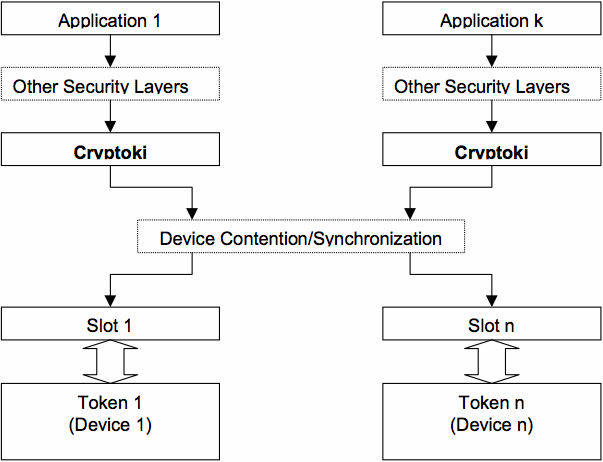
\includegraphics[scale=0.56]{images/general_cryptoki_model.png}
    \caption{Cryptoki Modell~\cite[S.14]{pkcs11}}
    \label{fig:cryptoki-model}
\end{figure}

Die Verbindung zu den Geräten (Tokens) wird über sogenannte "`Slots"' hergestellt. Obwohl in
der Grafik allen Slots ein Gerät zugewiesen ist, können sich mehrere Slots auch ein Gerät
teilen. Für das Anwendungsprogramm ist das letztlich irrelevant, ebenso wie die Art des
angeschlossenen Geräts.

\subparagraph{Logische Sicht auf Tokens}
Aus Sicht von Cryptoki ist ein Token irgendein Gerät, welches Objekte speichert und
kryptografische Funktionen ausführt~\cite[S.15]{pkcs11}, wobei ein Objekt Daten, einen
Schlüssel oder ein Zertifikat repräsentieren kann
(Abbildung~\ref{fig:cryptoki-object-hierarchy}).

\begin{figure}[ht]
    \centering
    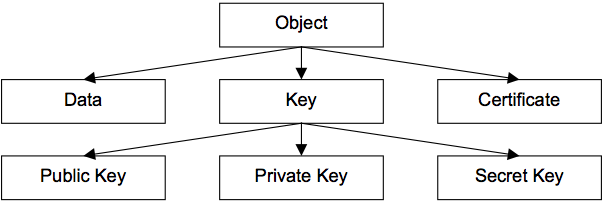
\includegraphics[scale=0.56]{images/cryptoki_object_hierarchy.png}
    \caption{Cryptokis Objekt-Hierarchie~\cite[S.15]{pkcs11}}
    \label{fig:cryptoki-object-hierarchy}
\end{figure}

Diese Objekt-Hierarchie stellt Cryptokis logische Sicht auf kryptografische Geräte dar.
Nicht jedes kryptografische Gerät arbeitet intern mit solchen Objekten und es ist die
Aufgabe der jeweiligen Cryptoki-Implementation, diese Implementierungsdetails in die
logische Sicht zu überführen.

\subparagraph{Benutzer}
Cryptoki definiert zwei Arten von Benutzern: den normalen Benutzer und den Security
Officer. Nur der normale Benutzer kann auf die privaten Daten des Tokens zugreifen,
allerdings erst nachdem er nach Eingabe eines PINs vom Security Officer authentifiziert
wurde. Inwiefern diese Benutzer in der konkreten Cryptoki-Implementation umgesetzt werden,
ist nicht Bestandteil des Standards. Die beiden Benutzer können verschiedene Personen
sein, es ist aber auch eine Implementierung möglich, in welcher eine Person beide Rollen
einnimmt. Ebenso ist die Art und Weise des benötigten PINs abhängig vom verwendeten
kryptografischen Gerät.

\paragraph{Verwendung von Cryptoki}
Dieser Abschnitt beschreibt die grundlegende Anwendung von Cryptoki.

\subparagraph{Zum Begriff "`Anwendungsprogramm"'}
Bis jetzt war von Anwendungsprogrammen als Benutzerschnittstellen die Rede, welche mit
einem Token kommunizieren müssen, um bspw. dessen kryptografischen Funktionen zu nützen.

Aus Sicht von Cryptoki ist ein Anwendungsprogramm ein einzelner Adressraum, inkl. aller
darin laufenden Threads. Durch den Aufruf der Cryptoki-Funktion \texttt{C\_Initialize()}
innerhalb eines Threads des Adressraums, wird die Applikation zu einer
"`Cryptoki-Applikation"'. Diese Sicht von Cryptoki bedeutet, dass ein mit \texttt{fork()}
gestarteter Kindprozess keinen Zugriff auf Tokens hat, solang er nicht selbst einen Aufruf
von \texttt{C\_Initialize()} macht.

\subparagraph{Sessions}
Um auf die Objekte und Funktionen eines an einem Slot angehängten Geräts zugreifen zu
können, muss mit Cryptoki zuerst eine Session gestartet werden, welche das
Anwendungsprogramme mit dem Slot und somit mit dem Gerät verbindet.

Es wird zwischen Read-Only- und Read-Write-Sessions unterschieden, wobei Token-Objekte nur
mit Read-Write-Sessions erstellt, bearbeitet und zerstört werden können. Weiter verfügen
Tokens über öffentliche und private Objekte. Zugriff auf die privaten Objekte des Tokens
sind nur möglich, wenn der normale Benutzer vom Security Officer authentifiziert wurde.

\subparagraph{Beenden der Verbindung}
Benötigt das Anwendunsprogramm das kryptografische Gerät nicht mehr, kann die Verbindung
durch Aufrufen von \\
\texttt{C\_Finalize()} beendet werden.

\subparagraph{Funktionsumfang}
Zwischen dem Erstellen der Sessions und dem Aufruf von \texttt{C\_Finalize()} kann das
Anwendungsprogramm mittels der von Cryptoki zur Verfügung gestellten Funktionen mit dem
kryptografischen Gerät kommunizieren. Dieser gesamte Funktionsumfang wird im Kapitel 11
von [PKCS11] detailliert beschrieben.

\subparagraph{Mechanismen}
[PKCS11] definiert in Kapitel 12 eine Menge von Mechanismen, welche kryptografische
Prozesse spezifizieren. Der Mechanismus \\
CKM\_RSA\_PKCS\_KEY\_PAIR\_GEN spezifiziert
beispielsweise die Generierung von RSA-Schlüsselpaaren. Diese Mechanismen stehen nicht
zwingend mit jedem kryptografischen Gerät zur Verfügung.

\subsection{PKCS \#12: Personal Information Exchange Syntax Standard}

\subsubsection{Einleitung}

\begin{table}[ht]
    \centering
    \begin{tabular}{|l|p{6.4cm}|} \hline
        Aktuelle Version des Standards & 1.1 \\\hline
        Datum & 27.10.2012 \\\hline
        Seitenzahl & 23 \\\hline
    \end{tabular}
\end{table}

\paragraph{Kurzbeschreibung RSA Laboratories}
\begin{quotation}
    \itshape This standard specifies a portable format for storing or transporting a
    user's private keys, certificates, miscellaneous secrets, etc.
\end{quotation}

\subsubsection{Zusammenfassung}

\paragraph{Scope}
Diese Definition standartisiert eine Syntax für den direkten Austausch von persönlichen
Identifikations Informationen wie z.B.:

\begin{itemize}
    \item Private Schlüssel
    \item Zertifikate
    \item Sonstige geheimen Daten
    \item Erweiterungen
\end{itemize}

Anwendungen, Browser, etc. welche diesen Standard unterstützen ermöglichen es Usern, ein
einzelnes Set von persönlichen Identitätsinformationen zu importieren und exportieren.
Dieser Standard kann als eine Erweiterung von PKCS \#8 angesehen werden. Zusätzlich bietet
man jedoch noch essentielle aber notwendige Identitätsinformationen samt privaten
Schlüssel an. Zudem ermöglicht man eine höhere Sicherheitsstufe durch den Einsatz von
public-key Verfahren sowie Integritätsschutz durch integrity modi.

PKCS\#12 kann sowohl in der Software als auch in der Hardware zum Einsatz kommen. Ein
Beispiel dazu ist die Sicherstellung der physikalischen Sicherheit für tamper-persistante
tokens, wie z.B. Smartcard / PCMCIA Treiber.

\paragraph{Einsatz}
Es werden zwei Sicherheitslevel unterstützt:
\begin{enumerate}
    \item (höchste Stufe) Public / Private Key Paar wo sowohl beim Sender und Empfänger
        zum Einsatz kommen für Verschlüsselung und Authentizitätsschutz (Integrität)
    \item (tiefere Stufe) Passwort-basierte privacy und integrity Modi, wenn keine public
        / private Key Paare zum Einsatz kommen können
\end{enumerate}

Mit diesen beiden Sicherheitslevel können insgesamt vier Kombinationen von
privacy/integrity Modi eingesetzt werden:

\begin{itemize}
    \item Privacy Modi:
        \begin{itemize}
            \item Public-key privacy Modus (Sender verschlüsselt mit dem öffentlichen
                Schlüssel des Empfängers. Der Empfänger entschlüsselt mit seinem privaten
                Schlüssel.)
            \item Password privacy Modus (Symmetrischer Schlüssel, welcher aus Username
                und Password erzeugt wird)
        \end{itemize}
    \item Integrity Modi:
        \begin{itemize}
            \item Public-key integrity Modus (Digitale Signatur mittels privatem Schlüssel
                des Senders. Wird beim Empfänger mit dem öffentlichen Schlüssel des
                Senders verifiziert.)
            \item Password integrity Modus (MAC abgeleitet aus einem geheimen \\
                Integritäts-Passwort)
        \end{itemize}
\end{itemize}

Für die Anwendung des Passwort-Integritäts Modus mit MAC wird HMAC verwendet. Gefordert
wird für die Hashfunktion SHA-1 und der MAC Schlüssel muss 160Bit betragen.

\paragraph{Richtlinien für die Wahl des Modus}
Grundsätzlich sind alle möglichen Kombinationen erlaubt. Es gibt allerdings gewisse Punkte
die beachtet werden sollten. Z.B. beim Einsatz von Password Privacy Modus sollte beim
Transport der privaten Schlüssel darauf geachtet werden, dass diese ausreichen
physikalisch geschützt werden. Zusammegefasst kann gesagt werden, dass Public-Key Modi für
Privacy sowohl auch für Integrity mit Password Modus kombiniert werden sollten.

\paragraph{Zuverlässige Public-Keys}
Asymmetrische Schlüsselpaare können in diesem Standard in zwei Arten genutzt werden:

\begin{itemize}
    \item Public-Key Privacy Modus
        \begin{itemize}
            \item Benötigt ein Schlüsselpaar für die Verschlüsslung (encryption)
        \end{itemize}
    \item Public-Key Integrity Modus
        \begin{itemize}
            \item Benötigt ein Schlüsselpaar für die Signature (signature)
        \end{itemize}
\end{itemize}

\paragraph{AuthenticatedSafe}
Jede konforme Plattform muss eine AuthenticatedSafe PDU’s (Protocol Data Unit) als PFX-PDU
gewrappte Einheit importieren und exportieren können. 

Die AuthenticatedSafe Einheit bestehen aus einer Sequenz von ContentInfo Einheiten. Diese
ContentInfo-Strukturen sind in PKCS\#7 beschrieben. Der Inhalts-Typ dieser
ContentInfo-Werte kann entweder Klartext (data), enveloped data (wenn Public-Key Privacy
Modus verwendet wird) oder encrypted data (wenn Password-Privacy Modus verwendet wird)
sein.

\begin{verbatim}
AuthenticatedSafe ::= SEQUENCE OF ContentInfo
    -- Data if unencrypted
    -- EncryptedData if password-encrypted
    -- EnvelopedData if public key-encrypted 
\end{verbatim}
Eine ContentInfo Einheit umfasst eine beliebige Sammlung von privaten Schlüssel, PKCS\#8
umhüllte private Schlüssel, Zertifikate, etc, welche als Werte des Typs SafeContents
gespeichert werden.

Der Aufbau einer AuthenticatedSafe PDU Einheit gewrappt als PFX-PDU Einheit:

\begin{verbatim}
PFX ::= SEQUENCE {
    version     Version    -- V3(3) for this version.
    authSafes   ContentInfo,    -- from PKCS #7 
        -- SignedData in public-key integrity mode
        -- Data in password integrity mode
    macData     MacData OPTIONAL
        -- present only in password integrity mode
}
\end{verbatim}

Der SafeContents-Typ besteht aus einer Sequenz aus SafeBags:

\begin{verbatim}
SafeContents ::= SEQUENCE OF SafeBag
\end{verbatim}

Ein SafeBag repräsentiert ein Stück Information, wie z.B. ein Schlüssel, ein Zertifikat
sowie optionale attribute. Jeder SafeBag wird durch einen Objekt Identifikator
identifiziert.

\begin{verbatim}
SafeBag ::= SEQUENCE {
    bagId BAG-TYPE.&id ({PKCS12BagSet})
    bagValue [0] EXPLICIT BAG-TYPE.&Type({PKCS12BagSet}{@bagId}),
    bagAttributes SET OF PKCS12Attribute OPTIONAL
}
\end{verbatim}

\subsection{PKCS \#13: Elliptische Kurven}

Die Kryptographie mit elliptischen Kurven erfährt eine zunehmende Popularität, da eine
vergleichbare Sicherheit zu etablierten Public Key Verfahren mit kleineren Schlüsseln
ermöglicht wird. Verbesserungen in der Implementierung wie der Erzeugung von elliptischen
Kurven machen das Verfahren praxistauglicher als bei seiner Einführung in den 1980-er
Jahren.

PCKS\#13 ist bis heute noch kein definitiver Standard. Der Standard ist noch immer in
Entwicklung. Der Standard soll die folgenden Aspekte der Kryptographie mit elliptischen
Kurven abdecken~\cite{pkcs13-proj}:

\begin{itemize}
    \item Parameter und Schlüssel Erzeugung und Validierung
    \item Digitale Signaturen
    \item Public Key Verschlüsselung
    \item Key Agreement (anstelle des verwundbaren anonymen Key-Exchanges wie z.Bsp.
        Diffie-Hellman)
    \item ASN.1 Syntax
    \item Überlegungen zur Sicherheit
\end{itemize}

Es sind bereits Standards in Arbeit, welche sich mit der Kryptographie mit elliptischen
Kurven befassen:
\begin{description}
    \item[ANSI X9.62] Ist ein in Entwicklung befindlicher Standard für digitale
        Signaturen.
    \item[ANSI X9.63 ] Ist ein in Entwicklung befindlicher Standard für Key Agreement.
    \item[IEEE P1363] Soll eine generelle Referenz für Public Key Verfahren verschiedener
        Techniken, inkl. elliptischer Kurven werden.
\end{description}

PKCS\#13 soll die anderen Standards vervollständigen, ein Profil der anderen Standards im
PKCS Format liefern und eine Anleitung für die Integration in andere PKCS Anwendungen (wie
beispielsweise PKCS\#7) bieten.

\subsubsection{Aktueller Umfang}

Zurzeit umfasst der Standard Grundlagen der folgenden Bereiche, welche allerdings keine
konkreten Implementierungen oder Standards nennt. Diese Themen können als Grundlagen der
Kryptographie mit elliptischen Kurven betrachtet werden.

\begin{description}
    \item[Functions] Grundlegende Definition einer Funktion: "`A function f from a set A
        to a set B assigns to each element a in A a unique element b in
        B."'~\cite{pkcs13-func}
    \item[Modular arithmetic] Grundlagen der modularen Arithmetik
    \item[Groups] Grundlagen der diskreten Mathematik ($\mathbb{Z}_p$ und
        $\mathbb{Z}_p^*$) in Bezug auf Gruppen.
    \item[Fields and rings] Ebenfalls mathematische Grundlagen.
    \item[Vector spaces and lattices] Behandelt die Grundlagen der linearen Algebra und
        der Vektorräume.
    \item[Boolean expressions] Die Betrachtung logischer Ausdrücke als Funktionen.
    \item[Time estimations and some complexitiy] Betrachtungen zur Komplexität.
\end{description}

Generell sind keine konkreten Vorgaben zu diesem Standard vorhanden. Zurzeit existiert
lediglich ein Vorschlag, welcher mögliche Key Agreement Schemes, Signature Schemes,
Encryption Schemes und Point Representations nennt.

\subsection{PKCS \#15: Cryptographic Token Information Syntax Standard}

\subsubsection{Einleitung}
\begin{table}[ht]
    \centering
    \begin{tabular}{|l|p{6.4cm}|} \hline
        Aktuelle Version des Standards & 1.1 \\\hline
        Datum & 16.05.2000 \\\hline
        Seitenzahl & 81 \\\hline
    \end{tabular}
\end{table}

\paragraph{Kurzbeschreibung RSA Laboratories}

\begin{quotation}
    \itshape PKCS \#15 establishes a standard that enables users in to use cryptographic
    tokens to identify themselves to multiple, standards-aware applications, regardless of
    the application's cryptoki (or other token interface) provider.
\end{quotation}

\subsubsection{Zusammenfassung}

\paragraph{Scope}
Diese Definition spezifiziert sowohl ein Datei- als auch ein Pfadformat, um
sicherheitsrelevante Informationen auf krypt. Tokens zu speichern. Die Realisierung kann
sowohl in Hardware für Smartcards, als auch in Software für virtuelle Smartcards erfolgen.
Allerdings ist dieser PKCS Standart veraltet und wird durch ISO/IEC 7816-15 abgelöst.

\paragraph{Ziele}
\begin{itemize}
    \item Platform Interoperabilität zwischen Komponenten welche auf verschiedenen
        Platformen laufen
    \item Produkte Unabhängigkeit (Verschiedenen Produkte verschiedener Hersteller können
        problemlos verwendent werden.)
    \item Applikationsunabhängigkeit (Es muss keine extra Applikations-Level-\\
        Software geschrieben werden um die Kompabilität zu gewährleisten.)
    \item Konsistenz von bestehender, verwendeter Standarts erhalten und diese wenn nötig
        weiter entwickeln
\end{itemize}

\paragraph{Anwendungsfall}
Ein Besitzer einer IC-Karte sollte diese überall einsetzen können, unabhängig auf welchem
System das Lesegerät betrieben wird. Es sollte ausschliesslich das Digitale-Zertifikat
korrekt einsetzen können und somit auf die Hauptaufgabe reduziert werden. Dieses Beispiel
umschreibt die oben erwähnten Ziele, wo am Schluss nicht das Hauptaugenmerk darauf
gerichtet wird, um was für Systeme / Komponenten es sich handelt. Es sollten alle einem
gemeinsamen Standart für die Verwaltung und den Einsatz von digitalen Zertifikaten folgen.

\paragraph{Profile für das Datenformat und Zugriffsbedingungen}
Diese Profil-Modelle definieren die Verzeichnisstruktur und Dateizugriffsbedingungen für
den Einsatz von Tokens. Sie sind nötig, um die Konformität zu gewähren. Das heisst, um ein
Token zu verwenden, benötigt man ein EID (Electronic Identification profile). Folgend ein
Beispiel aus der offiziellen RSA Dokumentation zu PKCS\#15:

\subparagraph{Verzeichnis Struktur}
\begin{itemize}
    \item MF: Master File
    \item EF: Elementary File
    \item DF: Directory File
\end{itemize}

\begin{figure}[ht]
    \centering
    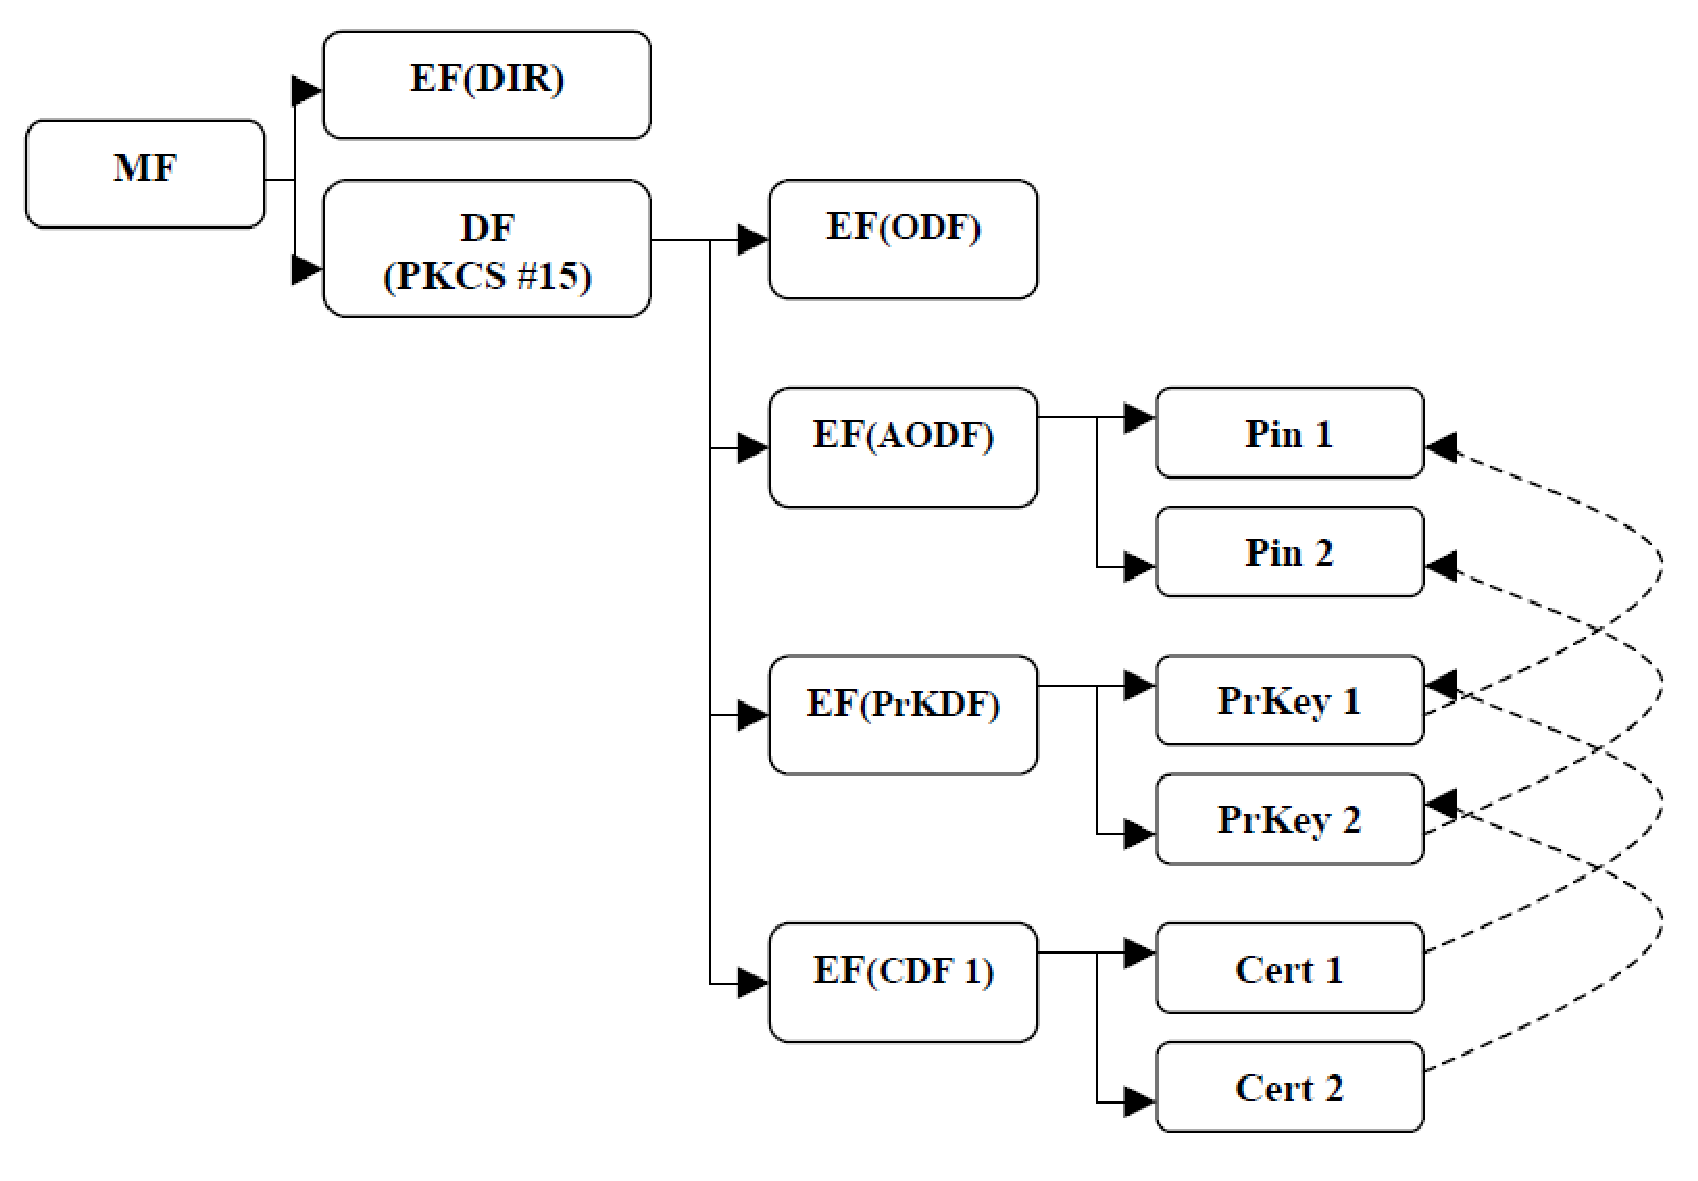
\includegraphics[scale=0.42]{images/layout-ef-df}
    \caption{Layout for the EFs and DFs for the profile}
    \label{fig:layout-ef-df}
\end{figure}

\subparagraph{Dateizugriffsbedingungen}
\begin{figure}[ht]
    \centering
    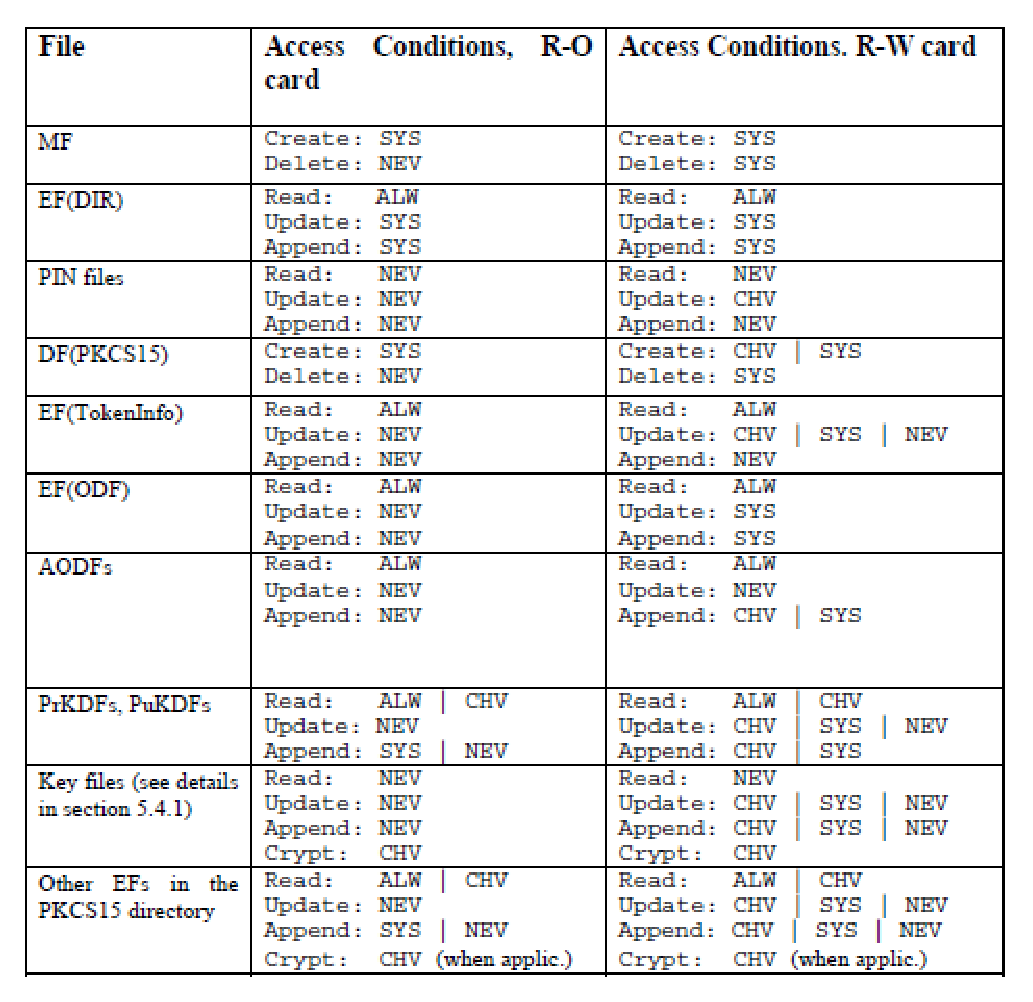
\includegraphics[scale=0.62]{images/access-cond-eid-profile}
    \caption{general access conditions for the EID Profile}
    \label{fig:access-cond-eid-profile}
\end{figure}

\FloatBarrier

\subparagraph{Anforderungen}

\paragraph{Private Schlüssel}
Es braucht mindestens 2 private Schlüssel in einem \\PKCS\#15-Token. Davon wird ein Schlüssel
sowohl für die Authorisierung wie auch Verschlüsselung benötigt. Der zweite Schlüssel wird
exklusiv für die Nachweisbarkeit oder für Digitale-Signatur verwendet.

\begin{itemize}
    \item \textbf{Privater Schlüssel 1: PrKey1} muss durch die \textbf{PIN1} erifiziert
        werden, bevor Verschlüsselungs-Operationen stattfinden können
    \item \textbf{Privater Schlüssel 2: PrKey2} muss durch die \textbf{PIN2} verifiziert
        werden, bevor jede Operation mit privaten Schlüsseln stattfinden können
\end{itemize}

\paragraph{Zertifikate}
Für jeden privaten Schlüssel muss mindestens 1 korrespondierender X509 Zertifikats-Typ im
Token gespeichert sein. Zudem muss auf dieses Zertifikat vom CDF(Certificate Directory
File) verwiesen werden.

\paragraph{Authentifizierungsobjekte}
Auf dem Token müssen mindestens zwei Authentifizierungsobjekte, für den Schutz von
privaten Objekten, vorhanden sein. Das zweite Authentifizierungsobekt, die PIN2, is
ausschliesslich für die Authentifizierung von Nachweisbarkeits-Objekte (non-repudiation)
zuständig. Zusätzlich muss die PIN2 nach jeder Operation mit privaten Schlüssel für die
Nachweisbarkeit, den Verfizierungsstatus auf "`nicht verifiziert"' setzen.


\FloatBarrier
\appendix
\renewcommand{\refname}{\section{Quellen}}
\begin{thebibliography}{}
    \bibitem[RSA-Lab]{rsa-lab} RSA Laboratories:
        \url{http://www.emc.com/domains/rsa/index.htm}, 1.1.2014
    \bibitem[KAL91]{kal91} Kalinski \& Burton S.: An Overview of the PKCS Standards, 1991
    \bibitem[PKCS-Standards]{pkcs-standards} RSA Laboratories: PUBLIC-KEY CRYPTOGRAPHY
        STANDARDS,
        \url{http://www.emc.com/emc-plus/rsa-labs/standards-initiatives/public-key-cryptography-standards.htm},
        1.1.2014
    \bibitem[PKCS1]{pkcs1} RSA Laboratories: PKCS\#1,
        \url{ftp://ftp.rsasecurity.com/pub/pkcs/pkcs-1/pkcs-1v2-1.pdf}
    \bibitem[PKCS3]{pkcs3} RSA Laboratories: PKCS \#3; Diffie-Hellman Key-Agreement
        Standard, 1993
    \bibitem[PKCS5]{pkcs5} RSA Laboratories: PKCS \#5; Password-Based Cryptography
        Standard Standard, 2000 (\url{http://www.ietf.org/rfc/rfc2898.txt})
    \bibitem[PKCS6]{pkcs6} RSA Laboratories: PKCS \#6; Extended- Certificate Syntax
        Standard,
        \url{http://www.emc.com/emc-plus/rsa-labs/standars-initiatives/pkcs-6-extended-certificate-syntax-standard.htm},
        1.1.2014
    \bibitem[PKCS7]{pkcs7} RSA Laboratories: PKCS \#7 Cryptographic Message Syntax Standard;
        1993
    \bibitem[PKCS8]{pkcs8} RSA Laboratories: PKCS \#8 Private-Key Information Syntax
        Specification Version 1.2, May 2008, \url{http://www.ietf.org/rfc/rfc5208.txt},
        1.1.2014
    \bibitem[PKCS9]{pkcs9} RSA Laboratories: PKCS \#9 v2.0; Selected Object Classes and
        Attribute Types; 2000
    \bibitem[PKCS10]{pkcs10} RSA Laboratories: PKCS \#10; Certification Request Syntax
        Standard, 2000
    \bibitem[PKCS11]{pkcs11} RSA Laboratories: PKCS \#11; Cryptographic Token Interface
        Standard, 2004
    \bibitem[PKCS12]{pkcs12} RSA Laboratories: PKCS \#12; Personal Information Exchange
        Syntax, 1999
    \bibitem[PKCS13]{pkcs13} RSA Laboratories: PKCS \#13: ELLIPTIC CURVE CRYPTOGRAPHY
        STANDARD
        \url{http://www.emc.com/emc-plus/rsa-labs/standards-initiatives/pkcs-13-elliptic-curve-cryptography-standard.htm}
    \bibitem[PKCS13-proj]{pkcs13-proj} RSA Laboratories: PKCS \#13 Project overview,
        \url{http://www.emc.com/emc-plus/rsa-labs/standards-initiatives/project-overview.htm},
        1.1.2013
    \bibitem[PKCS13-func]{pkcs13-func} RSA Laboratories: A.1 Functions,
        \url{http://www.emc.com/emc-plus/rsa-labs/standards-initiatives/functions.htm},
        1.1.2013
    \bibitem[PKCS15]{pkcs15} RSA Laboratories: PKCS \#15; Cryptographic Token Information
        Syntax Standard, 2000
\end{thebibliography}

\end{document}
